% ==== Document Class & Packages =====
\documentclass[12pt,hidelinks]{article}
\usepackage[norelsize, linesnumbered, ruled, lined, boxed, commentsnumbered]{algorithm2e}
	\usepackage[explicit]{titlesec}
	\usepackage[linesnumbered,ruled,vlined]{algorithm2e}
	\usepackage{indentfirst}
	\usepackage{lipsum}
    \usepackage{textcomp}
    \setcounter{secnumdepth}{6}
    \setcounter{tocdepth}{6}
    \usepackage{xpatch}
    \usepackage[utf8]{inputenc}
    \usepackage[utf8]{inputenc}
	\usepackage{titletoc}
	\usepackage{tocloft}
	\usepackage{charter}
	\usepackage[most]{tcolorbox}
	\usepackage{amsmath}
	\usepackage{graphicx}
	\usepackage{xcolor}
	\usepackage[T1]{fontenc}
	\usepackage[margin=20mm, a4paper, bindingoffset=4mm]{geometry}
	\usepackage{tikz,lipsum,lmodern}
	\usetikzlibrary{calc}
	\usepackage[english]{babel}
	\usepackage{fancyhdr}
	\usepackage{mathrsfs}
	\usepackage{empheq}
	\usepackage{fourier}% change to lmodern if fourier is no available
	\usepackage{wrapfig}
	\usepackage{fancyref}
	\usepackage{hyperref}
	\usepackage{cleveref}
	\usepackage{listings}
	\usepackage{varwidth}
	\usepackage{longfbox}
	\usepackage{geometry}
	\usepackage{marginnote}
    \usepackage{soul}
	\tcbuselibrary{theorems}
	\tcbuselibrary{breakable, skins}
	\tcbuselibrary{listings, documentation}
	\geometry{
		a4paper,
		left=33mm,
		right=33mm,
		top=20mm}
		
\SetKwInput{KwInput}{Input}                % Set the Input
\SetKwInput{KwOutput}{Output}              % set the Output


\renewcommand{\theparagraph}{\Alph{paragraph}}
\newcommand\mycommfont[1]{\footnotesize\ttfamily\textcolor{blue}{#1}}
\SetCommentSty{mycommfont}

\makeatletter
\xpatchcmd{\thesubparagraph}{%
\theparagraph.\@arabic\c@subparagraph}{%
\arabic{subparagraph}\textsuperscript{}}{}{}
\makeatletter         
\def\@maketitle{
\begin{center}
\includegraphics[width=0.5\linewidth]{ECN_logo.png}

{\Large \bfseries \sffamily \@title }\\[4ex] 
{\Large  \@author}\\[4ex] 

\end{center}}
\makeatother
% ========= Path to images ============
%   - Direct the computer on the path 
% 	  to the folder containg the images
% =====================================
\graphicspath{{./images/}}
% ============= Macros ================
\newcommand{\fillin}{\underline{\hspace{.75in}}{\;}}
\newcommand{\solution}{\textcolor{mordantred19}{Solution:}}
\setlength{\parindent}{0pt}
\addto{\captionsenglish}{\renewcommand*{\contentsname}{Table of Contents}}
\linespread{1.2}
% ======== Footers & Headers ==========
\cfoot{\thepage}
\chead{}\rhead{}\lhead{}
% =====================================
\renewcommand{\thesection}{\arabic{section}}
\newcommand\sectionnumfont{% font specification for the number
	\fontsize{115}{70}\color{myblueii}\selectfont}
\newcommand\sectionnamefont{% font specification for the name "PART"
	\fontsize{115}{70}\color{white}\scshape\small\bfseries }
% ============= Colors ================
% ----- Red -----
\definecolor{mordantred19}{rgb}{0.68, 0.05, 0.0}
% ----- Blue -----
\definecolor{st.patrick\'sblue}{rgb}{0.14, 0.16, 0.48}
\definecolor{teal}{rgb}{0.0, 0.5, 0.5}
\definecolor{beaublue}{rgb}{0.74, 0.83, 0.9}
\definecolor{mybluei}{RGB}{0,173,239}
\definecolor{myblueii}{RGB}{63,200,244}
\definecolor{myblueiii}{RGB}{199,234,253}
% ---- Yellow ----
\definecolor{blond}{rgb}{0.98, 0.94, 0.75}
\definecolor{cream}{rgb}{1.0, 0.99, 0.82}
% ----- Green ------
\definecolor{emerald}{rgb}{0.31, 0.78, 0.47}
\definecolor{darkspringgreen}{rgb}{0.09, 0.45, 0.27}
% ---- White -----
\definecolor{ghostwhite}{rgb}{0.97, 0.97, 1.0}
\definecolor{splashedwhite}{rgb}{1.0, 0.99, 1.0}
% ---- Grey -----
\definecolor{whitesmoke}{rgb}{0.96, 0.96, 0.96}
\definecolor{lightgray}{rgb}{0.92, 0.92, 0.92}
\definecolor{floralwhite}{rgb}{1.0, 0.98, 0.94}
% ========= Part Format ==========
\titleformat{\section}
{\normalfont\huge\filleft}
{}
{20pt}
{\begin{tikzpicture}[remember picture,overlay]
	\fill[myblueiii] 
	(current page.north west) rectangle ([yshift=-7cm]current page.north east);   
\node[
	fill=mybluei,
	text width=2\paperwidth,
	rounded corners=3cm,
	text depth=9cm,
	anchor=center,
	inner sep=0pt] at (current page.north east) (parttop)
	{\thepart};%
\node[
	anchor=south east,
	inner sep=0pt,
	outer sep=0pt] (partnum) at ([xshift=-20pt]parttop.south) 
	{\sectionnumfont\thesection};
\node[
	anchor=south,
	inner sep=0pt] (partname) at ([yshift=2pt]partnum.south)   
	{\sectionnamefont SECTION};
\node[
	anchor=north east,
	align=right,
	inner xsep=0pt] at ([yshift=-0.5cm]partname.east|-partnum.south) 
	{\parbox{.7\textwidth}{\raggedleft#1}};
\end{tikzpicture}%
}
% ========= Hyper Ref ===========
\hypersetup{
	colorlinks,
	linkcolor={red!50!black},
	citecolor={blue!50!black},
	urlcolor={blue!80!black}
}
% ========= Example Boxes =============
\tcbset{
	defstyle/.style={
		fonttitle=\bfseries\upshape, 
		fontupper=\slshape,
		arc=0mm, 
		beamer,
		colback=blue!5!white,
		colframe=blue!75!black},
	theostyle/.style={
		fonttitle=\bfseries\upshape, 
		fontupper=\slshape,
		colback=red!10!white,
		colframe=red!75!black},
	visualstyle/.style={
		height=6.5cm,
		breakable,
		enhanced,
		leftrule=0pt,
		rightrule=0pt,
		bottomrule=0pt,
		outer arc=0pt,
		arc=0pt,
		colframe=mordantred19,
		colback=lightgray,
		attach boxed title to top left,
		boxed title style={
			colback=mordantred19,
			outer arc=0pt,
			arc=0pt,
			top=3pt,
			bottom=3pt,
		},
		fonttitle=\sffamily,},
	discussionstyle/.style={
		height=6.5cm,
		breakable,
		enhanced,
		rightrule=0pt,
		toprule=0pt,
		outer arc=0pt,
		arc=0pt,
		colframe=mordantred19,
		colback=lightgray,
		attach boxed title to top left,
		boxed title style={
			colback=mordantred19,
			outer arc=0pt,
			arc=0pt,
			top=3pt,
			bottom=3pt,
		},
		fonttitle=\sffamily},
	mystyle/.style={
		height=6.5cm,
		breakable,
		enhanced,
		rightrule=0pt,
		leftrule=0pt,
		bottomrule=0pt,
		outer arc=0pt,
		arc=0pt,
		colframe=mordantred19,
		colback=lightgray,
		attach boxed title to top left,
		boxed title style={
			colback=mordantred19,
			outer arc=0pt,
			arc=0pt,
			top=3pt,
			bottom=3pt,
		},
		fonttitle=\sffamily},
	aastyle/.style={
			height=3.5cm,
			enhanced,
			colframe=teal,
			colback=lightgray,
			colbacktitle=floralwhite,
			fonttitle=\bfseries,
			coltitle=black,
		attach boxed title to top center={
	  		yshift=-0.25mm-\tcboxedtitleheight/2,
	   		yshifttext=2mm-\tcboxedtitleheight/2}, 
		boxed title style={boxrule=0.5mm,
			frame code={ \path[tcb fill frame] ([xshift=-4mm]frame.west)
				-- (frame.north west) -- (frame.north east) -- ([xshift=4mm]frame.east)
				-- (frame.south east) -- (frame.south west) -- cycle; },
			interior code={ 
				\path[tcb fill interior] ([xshift=-2mm]interior.west)
				-- (interior.north west) -- (interior.north east)
				-- ([xshift=2mm]interior.east) -- (interior.south east) -- (interior.south west)
				-- cycle;} }
				},
	examstyle/.style={
		height=9.5cm,
		breakable,
		enhanced,
		rightrule=0pt,
		leftrule=0pt,
		bottomrule=0pt,
		outer arc=0pt,
		arc=0pt,
		colframe=mordantred19,
		colback=lightgray,
		attach boxed title to top left,
		boxed title style={
			colback=mordantred19,
			outer arc=0pt,
			arc=0pt,
			top=3pt,
			bottom=3pt,
		},
		fonttitle=\sffamily},
	doc head command={
		interior style={
			fill,
			left color=yellow!20!white, 
			right color=white}},
	doc head environment={
		boxsep=4pt,
		arc=2pt,
		colback=yellow!30!white,
		},
	doclang/environment content=text
}
% ============= Boxes ================
\newtcolorbox[auto counter,number within=section]{example}[1][]{
	mystyle,
	title=Example~\thetcbcounter,
	overlay unbroken and first={
		\path
		let
		\p1=(title.north east),
		\p2=(frame.north east)
		in
		node[anchor=
			west,
			font=\sffamily,
			color=st.patrick\'sblue,
			text width=\x2-\x1] 
		at (title.east) {#1};
	}
}
\newtcolorbox[auto counter,number within=section]{longexample}[1][]{
	examstyle,
	title=Example~\thetcbcounter,
	overlay unbroken and first={
		\path
		let
		\p1=(title.north east),
		\p2=(frame.north east)
		in
		node[anchor=
		west,
		font=\sffamily,
		color=st.patrick\'sblue,
		text width=\x2-\x1] 
		at (title.east) {#1};
	}
}
\newtcolorbox[auto counter,number within=section]{example2}[1][]{
	aastyle,
	title=Example~\thetcbcounter,{}
}
\newtcolorbox[auto counter,number within=section]{discussion}[1][]{
	discussionstyle,
	title=Discussion~\thetcbcounter,
	overlay unbroken and first={
		\path
		let
		\p1=(title.north east),
		\p2=(frame.north east)
		in
		node[anchor=
		west,
		font=\sffamily,
		color=st.patrick\'sblue,
		text width=\x2-\x1] 
		at (title.east) {#1};
	}
}
\newtcolorbox[auto counter,number within=section]{visualization}[1][]{
	visualstyle,
	title=Visualization~\thetcbcounter,
	overlay unbroken and first={
		\path
		let
		\p1=(title.north east),
		\p2=(frame.north east)
		in
		node[anchor=
		west,
		font=\sffamily,
		color=st.patrick\'sblue,
		text width=\x2-\x1] 
		at (title.east) {#1};
	}
}
% --------- Theorems ---------
\newtcbtheorem[number within=subsection,crefname={definition}{definitions}]%
	{Definition}{Definition}{defstyle}{def}%
\newtcbtheorem[use counter from=Definition,crefname={theorem}{theorems}]%
	{Theorem}{Theorem}{theostyle}{theo}
	%
\newtcbtheorem[use counter from=Definition]{theo}{Theorem}%
{
	theorem style=plain,
	enhanced,
	colframe=blue!50!black,
	colback=yellow!20!white,
	coltitle=red!50!black,
	fonttitle=\upshape\bfseries,
	fontupper=\itshape,
	drop fuzzy shadow=blue!50!black!50!white,
	boxrule=0.4pt}{theo}
\newtcbtheorem[use counter from=Definition]{DashedDefinition}{Definition}%
 {
 	enhanced,
 	frame empty,
 	interior empty,
 	colframe=darkspringgreen!50!white,
	coltitle=darkspringgreen!50!black,
	fonttitle=\bfseries,
	colbacktitle=darkspringgreen!15!white,
	borderline={0.5mm}{0mm}{darkspringgreen!15!white},
	borderline={0.5mm}{0mm}{darkspringgreen!50!white,dashed},
	attach boxed title to top center={yshift=-2mm},
	boxed title style={boxrule=0.4pt},
	varwidth boxed title}{theo}
%%%%%%%%%%%%%%%%%%%%%%%%%%%%%%%%%%%%%%%%
\newtcblisting[auto counter,number within=section]{disexam}{
	skin=bicolor,
	colback=white!30!beaublue,
	colbacklower=white,
	colframe=black,
	before skip=\medskipamount,
	after skip=\medskipamount,
	fontlower=\footnotesize,
	listing options={style=tcblatex,texcsstyle=*\color{red!70!black}},}
%%%%%%%%%%%%%%%%%%%%%%%%%%%%%%%%%%%%%%%

\begin{document}
\begin{titlepage}
	\centering % Center everything on the title page
	\scshape % Use small caps for all text on the title page
	\vspace*{1.5\baselineskip} % White space at the top of the page
% ===================
%	Title Section 	
% ===================

	\rule{13cm}{1.6pt}\vspace*{-\baselineskip}\vspace*{2pt} % Thick horizontal rule
	\rule{13cm}{0.4pt} % Thin horizontal rule
	
		\vspace{0.75\baselineskip} % Whitespace above the title
% ========== Title ===============	
	{	\Huge M2 CORO-ERTS project 2021-2022 :
	 EDF validation \&  \linebreak ED-H implementation over Xenomai\\	}
	 
% ======================================
		\vspace{0.75\baselineskip} % Whitespace below the title
	\rule{13cm}{0.4pt}\vspace*{-\baselineskip}\vspace{3.2pt} % Thin horizontal rule
	\rule{13cm}{1.6pt} % Thick horizontal rule
	
		\vspace{1.75\baselineskip} % Whitespace after the title block
% =================
%	Information	
% =================
	\author \textbf Advisor: Audrey Queudet \\
	\small Debus Alexy, Rayella Niranjan \\
	

	\begin{figure}[h]
    \centering
	
\includegraphics[scale=0.25]{Logo_ECN.png}
	%ADD the line below to add the figure in the "List of Figures" section 
	%\caption[simplified title]{complete title}
	\end{figure}
	
\vfill
\small{\noindent \textbf{Support} \vspace{-3mm}\\
\noindent \rule{3.3cm}{0.5pt} \\
if you encounter any problem, please reach us by mail \newline \url{alexy.Debus@eleves.ec-nantes.fr}, \\ \vspace{1mm}
	\end{titlepage}
\newpage

%%%%%%%%%%%%%%%%%%%%%%%%%%%%%%%%%%%%%%%%%%%%%%%%%%%%%%%%%%%
\tableofcontents
\vfill
\small{\noindent \textbf{About this document} \vspace{-3mm}\\
\noindent \rule{3.3cm}{0.5pt} \\
This document is intended for educational use within ECN. Consequently, its content is free of rights.
\newpage
\newgeometry{
	left=29mm, 
	right=29mm, 
	top=20mm, 
	bottom=15mm}
%%%%%%%%%%%%%%%%%%%%%%%%%%%%%%%%%%%%%%%%%%%%%%%%%%%%%%%%%%%
\section{Project organization}
\vspace{4cm}
    


%===============================

	\subsection{Introduction}
    \newline
    To work efficiently in this project, we have decide to divide the projects in sprints. Each sprints has an average 2 weeks length. For each sprint, specific task and milestones are pre-defined in order to break the project schedule into smaller block of time in which smaller objectives must be achieved.
    
    On october the 15th, we meet Ms.Queudet, the advisor of this project. She gave the interest of the project : Put into applications a dynamic-priority energy aware scheduling policy, I mean ED-H, through the use of a RT (Real-time) kernel.
    
    To perform this, we will have a dual kernel configurations : a Linux non RT kernel and a Xenomai RT kernel (Cobalt).
    
    On top of that, a master student had previously integrated EDF policy into Xenomai but no tests have been executed.
    
    So to sum up, the aim will be to assert EDF integration over Xenomai then integrate ED-H policy without affecting integrity of other scheduling policies (round-robin and EDF). 
    
    \subsection{Objectives}
    
    Below is a list of the primary objectives for the project :
    \begin{enumerate}
        \item Installation of modified Xenomai and validation for EDF integration

        Metric : \begin{itemize}
            \item Report for modifications added to have a functional installation
            \item Tests to validate EDF source code over Xenomai
        \end{itemize}
        
        \item Development of  a Linux module to grab battery information and send them to Cobalt kernel

        Metric : \begin{itemize}
            \item Guideline for the creation/use of the Linux module
            \item Source code for the Linux battery module​
        \end{itemize}

        \item ED-H implementation over Xenomai and validation 

        Metric : \begin{itemize}
            \item Source code for ED-H implementation over Xenomai 
            \item Source code for a fake linux battery module
        \end{itemize}
        
        \item Redaction of the final report, PWP presentation, handle git repositories 

    \end{enumerate}
    
    
	\vspace{-1.5mm}
\newpage
%%%%%%%%%%%%%%%%%%%%%%%%%%%%%%%%%%%%%%%%%%%%%%%%%%%%%%%%%%%
\section{Validation for EDF policy}
\vspace{4cm}

In this section, we will descibe the entire process to validate the EDF policy developped over Xenomai (refer to the \href{https://github.com/skyultime/Xenomai-EDH/commit/37aed321405df633a39f17e16ad50599cadb9ed9}{github repository} for EDF policy source code 

    \subsection{Cobalt core installation with dynamic priority policy}
    
    The first step was to compilate/install the cobalt core (I mean the dual-core configuration) for Xenomai 3.1.\newline \newline
    In order to do this, you can follow the installation manual available \href{Doc/CobaltCoreXenomaiInstallation/XenomaiEDF-installationGuide-1.pdf}{here}, respecting few modifications listed below to ensure a proper installation :\newline
    
    If you want to have Xenomai with EDF policy only :
    \begin{itemize}
       \item Replace the github link: \href{https://github.com/BraveMole/Xenomai-EDF.git}{https://github.com/BraveMole/Xenomai-EDF.git} with this one : \href{https://github.com/skyultime/Xenomai-EDH.git}{https://github.com/skyultime/Xenomai-EDH.git} Be sure to move on branch EDFpolicyV1.0 with the following command : \textbf{git checkout EDFpolicyV1.0}
       
       \item To configure the Kernel (cmd \textbf{make menu-config}), load directly the .config file available \href{https://github.com/skyultime/M2_ERTS_Project_Xenomai_edh/tree/dev/SourceCode/Patch/LinuxConfigFiles}{here} (the ipipe patch is also available in the same location if needed)
       
    \end{itemize}
    
    If you want to have Xenomai with EDF and EDH policy :
     \begin{itemize}
       \item Replace the github link : \href{https://github.com/BraveMole/Xenomai-EDF.git}{https://github.com/BraveMole/Xenomai-EDF.git} with this one : \href{https://github.com/skyultime/Xenomai-EDH.git}{https://github.com/skyultime/Xenomai-EDH.git}. Be sure to move on branch final\_version with the following command : \textbf{git checkout final\_version}
       
       \item To configure the Kernel (cmd \textbf{make menu-config}), load directly the .config file available \href{https://github.com/skyultime/M2_ERTS_Project_Xenomai_edh/tree/dev/SourceCode/Patch/LinuxConfigFiles}{here} (the ipipe patch is also available in the same location if needed)
       
    \end{itemize}
    
    In case you want to start from scratch and integrate\cite{EDF}DF or EDH policy in default Xenomai 3.1 git repository, you can use the default repository : \href{https://github.com/openil/Xenomai-3.git}{https://github.com/openil/Xenomai-3.git} and add patch available \href{https://github.com/skyultime/M2_ERTS_Project_Xenomai_edh/tree/dev/SourceCode/Patch}{here} (1 patch for EDF and 1 additional patch for EDH)

    \subsection{EDF Source code modification}
        
        In order to view details of implementation for EDF policy integration over Xenomai 3.1, you can have a look to the EDF.patch file available \href{https://github.com/skyultime/M2_ERTS_Project_Xenomai_edh/blob/dev/SourceCode/Patch/EDF.patch}{here}

        Here is the list of modified files:
        
        Major modifications :
        \begin{itemize}
            \item kernel/cobalt/sched-dyna.c
            \item kernel/cobalt/sched.c
            \item kernel/cobalt/posix/thread.c
            \item kernel/cobalt/thread.c
            \item lib/alchemy/task.c
            \item include/cobalt/kernel/sched-dyna.h
            \item include/cobalt/kernel/sched.h
            \item include/cobalt/kernel/thread.h
            \item include/alchemy/task.h
        \end{itemize}
        
        Minor modifications
        \begin{itemize}
            \item         include/mercury/boilerplate/sched.h
            \item kernel/cobalt/posix/sched.c
            \item include/cobalt/uapi/sched.h
            \item include/cobalt/kernel/schedparam.h
            \item include/cobalt/kernel/list.h
            \item include/cobalt/kernel/schedqueue.h
            \item lib/copperplate/internal.c
            \item lib/copperplate/threadobj.c
        \end{itemize}

    On top of that, the purpose of the last commit related to EDF policy implementation (see \href{https://github.com/skyultime/Xenomai-EDH/commit/37aed321405df633a39f17e16ad50599cadb9ed9}{here}) is only to have a proper compilation of Xenomai source code files without warning/errors.\newline

    Basically, the implementation of the EDF policy over Xenomai relies on :
    \begin{itemize}
        \item The creation of a new xnsched\_class, called \textbf{dyna}, to host tasks scheduled using the EDF policy. (cf. file sched\_dyna.c available \href{https://github.com/skyultime/Xenomai-EDH/blob/final_version/kernel/cobalt/sched-dyna.c}{here})
        \item Creation of function \textbf{rt\_task\_create\_dyna} to pass the deadline of the task. (cf figure below)


    \begin{figure}[ht]
        \centering
        \begin{minipage}{0.45\textwidth}
            \centering
            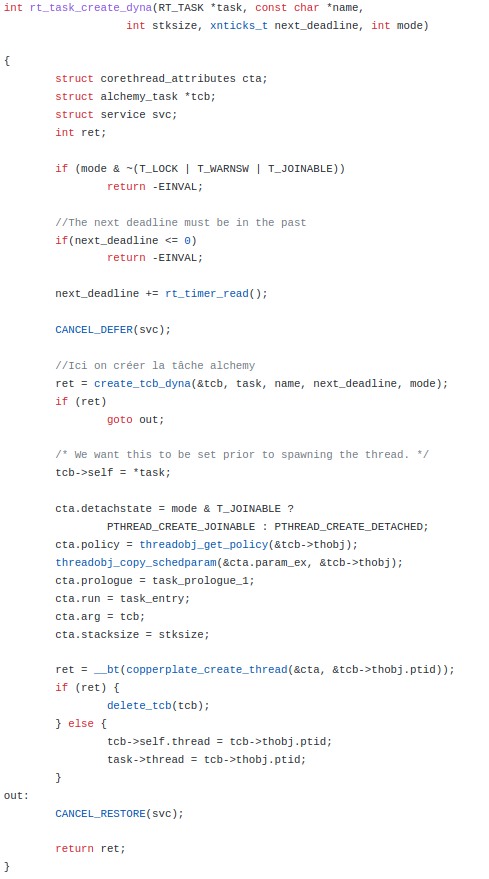
\includegraphics[width=0.9\textwidth]{rt_task_create_dyna_func.png} % first figure itself
            \caption{Function rt\_task\_create\_dyna}
        \end{minipage}\hfill
        \begin{minipage}{0.45\textwidth}
            \centering
            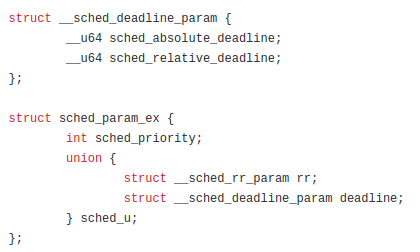
\includegraphics[width=0.9\textwidth]{struct __sched_deadline_param.png} % second figure itself
            \caption{struct sched\_deadline\_param for EDF policy}
        \end{minipage}
    \end{figure} \newline
    
    \newpage
    \item To enqueue a task in a list using round-robin policy, we need to pay attention to the priority of each task. However when we enqueue a task in a list using EDF policy (or EDH policy as well), we need to pay attention to the deadline of each task. While the value 0 correspond to a lowest priority when using round-robin policy (I mean the task with the lowest priority), a task with a small deadline will be the first queued element (lower is the deadline value, higher is the priority of the task).\newline Figures below demonstrate how to integrate these modifications. (in folder include /include/cobalt/kernel, cf. \href{https://github.com/skyultime/Xenomai-EDH/tree/EDFpolicyV1.0/include/cobalt/kernel}{here})
    
    \end{itemize}
        	
    \begin{figure}[ht]
    \centering
	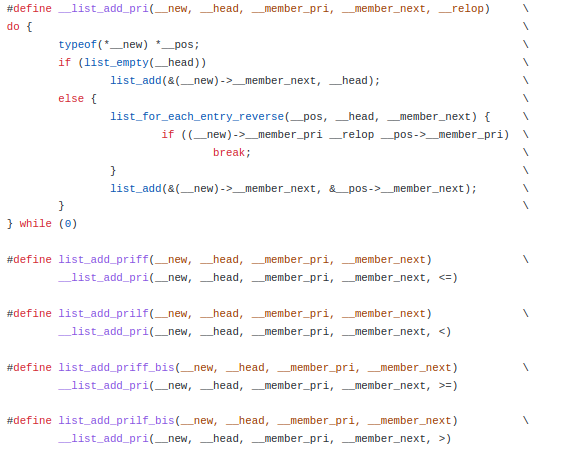
\includegraphics[scale=0.5]{list.png}
	\caption{File list.h}
	\end{figure} \newline
    
        \begin{figure}
        \centering
        \begin{minipage}{0.45\textwidth}
            \centering
            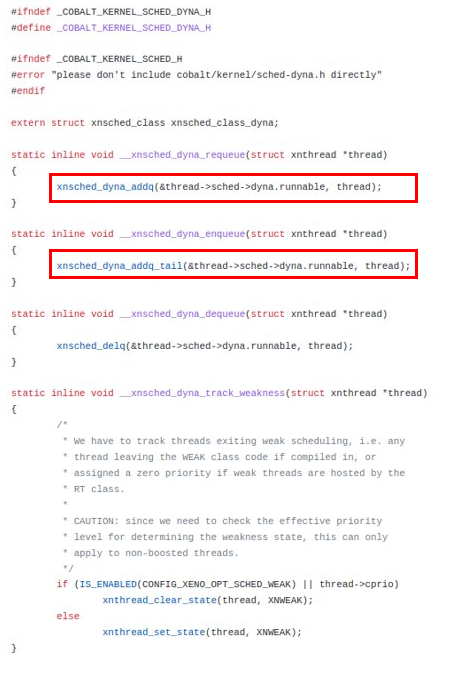
\includegraphics[width=1\textwidth]{sched_dyna.png} % first figure itself
            \caption{File sched\_dyna.h}
        \end{minipage}\hfill
        \begin{minipage}{0.45\textwidth}
            \centering
            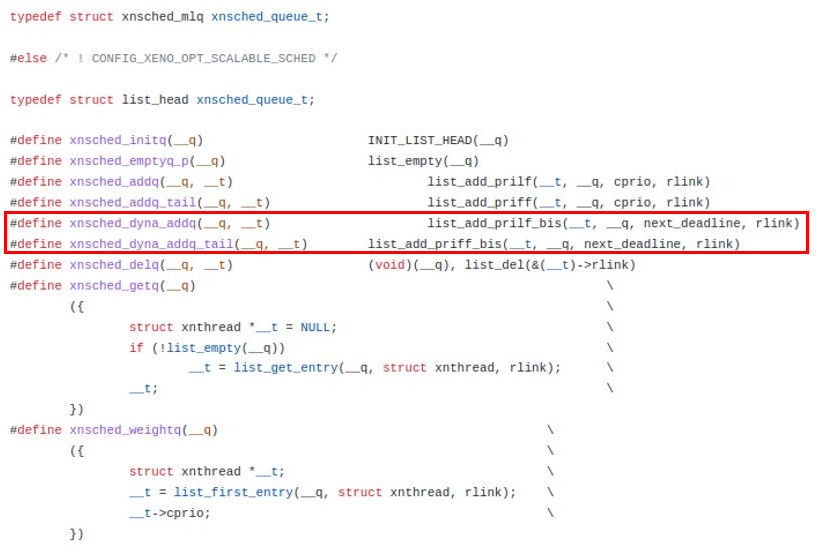
\includegraphics[width=1\textwidth]{schedparam.png} % second figure itself
            \caption{File schedparam.h}
        \end{minipage}
    \end{figure}
    


    \newpage
    \subsection{EDF Source code Validation} \label{validation}
    
    Now, let's have a look to the validation process to ensure the EDF policy is working well over Xenomai through simple examples.
    
    The source code dedicated to create/start a pre-defined number of real-time tasks scheduled with EDF policy is available \href{https://github.com/skyultime/M2_ERTS_Project_Xenomai_edh/tree/main/Tests/EDFonXenomai/edfAsserts}{here}.
    
    A first important thing to do in order to compilate source code using Xenomai Alchemy API is to define the CFLAGS,LDFLAGS and CC Flags as shown below :
    
    \begin{figure}[ht]
        \centering
        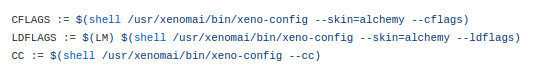
\includegraphics[scale=1]{flagsDefMakefile.png}
        \caption{Define flags in Makefile.h}
	\end{figure} \newline
    
    Then the architecture of the source code, \textbf{edfAsserts} is really simple.\newline
    Indeed we have :
    \begin{itemize}
        \item the main
        \item the listener (file \textbf{listener.c/.h}
        \item the controller (file \textbf{loop_task.c/.h}
    \end{itemize}
    
    The execution process is really simple:
    \begin{enumerate}
        \item follow the README.md to execute the ./EDFtest binary (link \href{https://github.com/skyultime/M2_ERTS_Project_Xenomai_edh/tree/main/Tests/EDFonXenomai/edfAsserts}{here})
        \item Choose to use dynamic priority,enter the number of tasks and desired parameters for each task in the terminal
        \item Oberve the results (also display in the terminal).
    
    \end{enumerate}
        
        To validate our results (in order to ensure EDF policy is working well over Xenomai), the 1st step could be to execute again our binary but this time, we will decide to use fixed priority policy (basically here the dafult one is the round-robin policy) and then compare both previous results with EDF and new results with round-robin.\newline
        
        Here is one example with the following parameters :
        \begin{table}[ht]
        \centering
        \begin{tabular}{|l|l|l|}
        \hline
        Tasks&Deadlines&WCET\\\hline
        Task 1&70ms&20ms\\\hline
        Task 2&90ms&20ms\\\hline
        Task 3&110ms&20ms\\\hline
        \end{tabular} 
        \caption{Test case n°1 to validate EDF policy implementation over Xenomai (Period = Deadline}
        \label{tab1}
        \end{table}

        First we could use these values and observe the behaviour with EDF policy and Round-robin policy. Below are the parameters we entered when executing the binary EDF test (keep in mind the conversion rate => 70 000 000 units = 70 ms):
        
         \begin{figure}[ht]
            \centering
            \begin{minipage}{0.4\textwidth}
                \centering
                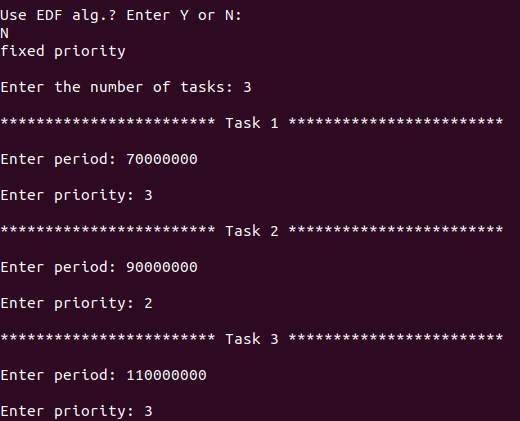
\includegraphics[width=1.25\textwidth]{paramFixed.png} % first figure itself
                \caption{Param. for fixed policy}
            \end{minipage}\hfill
            \begin{minipage}{0.4\textwidth}
                \centering
                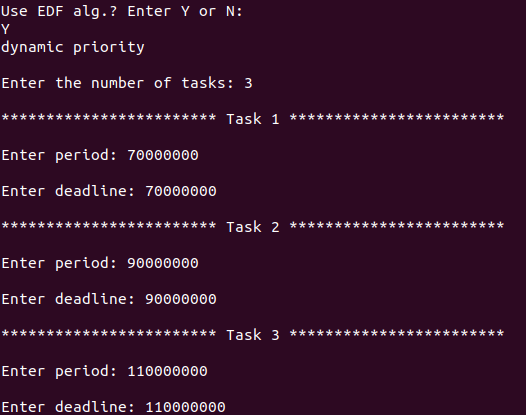
\includegraphics[width=1.3\textwidth]{paramDynamic.png} % second figure itself
                \caption{Param. for EDF policy}
            \end{minipage}
        \end{figure} \newline
        
        Then we can compare the 2 execution. The figure 8 exhibits the 3 tasks scheduled with round-robin policy(which could be here seen as a Rate Monotonic policy here because we assign a different priority to each RT task). There is no preemption occuring and the priority of execution is directly linked to the priority of each tasks as describes in table 1.\newline
        The figure 9 exhibits the 3 tasks scheduled with EDF policy. We can indeed clearly see the differences with figures 8. We can observe preemptions and tasks being scheduled according to their deadlines.
        
        \begin{figure}[ht]
            \centering
            \begin{minipage}{0.45\textwidth}
                \hspace{-2.5cm}
                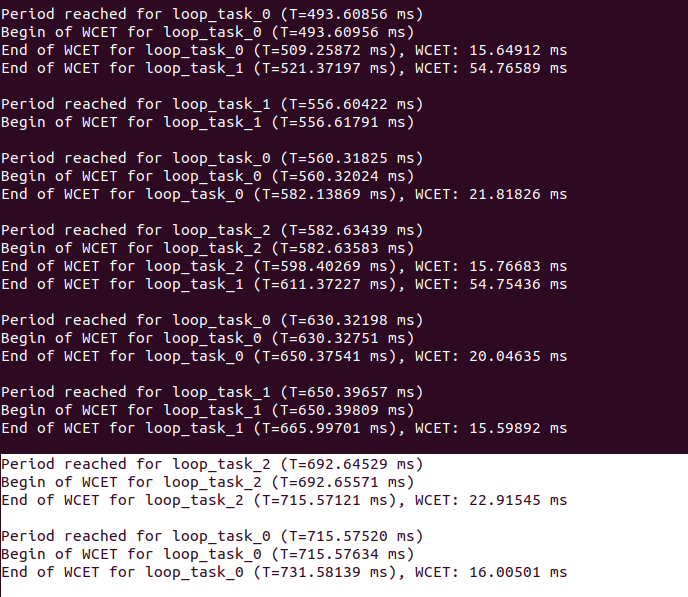
\includegraphics[width=1.4\textwidth]{FixedWithoutPreemption.png} % first figure itself
                \caption{Fixed policy without preemption}
            \end{minipage}\hfill
            \begin{minipage}{0.45\textwidth}
                \hspace{-1cm}
                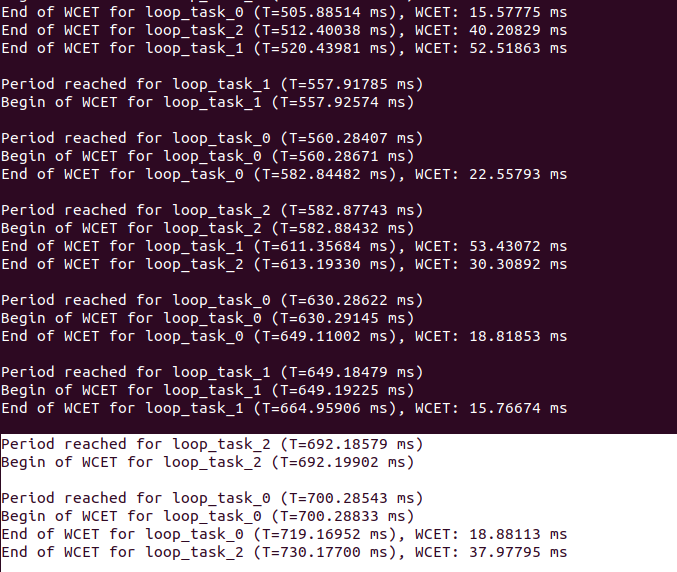
\includegraphics[width=1.43\textwidth]{DynaWithPreemption.png} % second figure itself
                \caption{EDF policy with preemption}
            \end{minipage}
        \end{figure} \newline

        
        In order to clearly observe preemptions (and so be sure to have a proper EDF scheduling activity), we can directly compare our results with a tool, called Cheddar. Cheddar allows you to model software architectures of real-time systems in order to check their schedulability (available \href{http://beru.univ-brest.fr/cheddar/#RefDownloadRelease}{here}). 
        
        Let's simulate with Cheddar using parameters define in table 1 (examples and configuration files for Cheddar are available \href{https://github.com/skyultime/M2_ERTS_Project_Xenomai_edh/tree/main/Tests/EDFonXenomai/EDF_Problem}{here} if needed) and let's compare with what we obtained using EDF policy over Xenomai:

        \begin{itemize}
            \item In this first view, the task T2 is executing. On both view (Cheddar on the left, Xenomai on the right) at T= 840 ms , T1 which has a shortest deadline than T2 is preempted it.
            
            \begin{figure}[h]
                \hspace*{-2cm}   
                \centering
                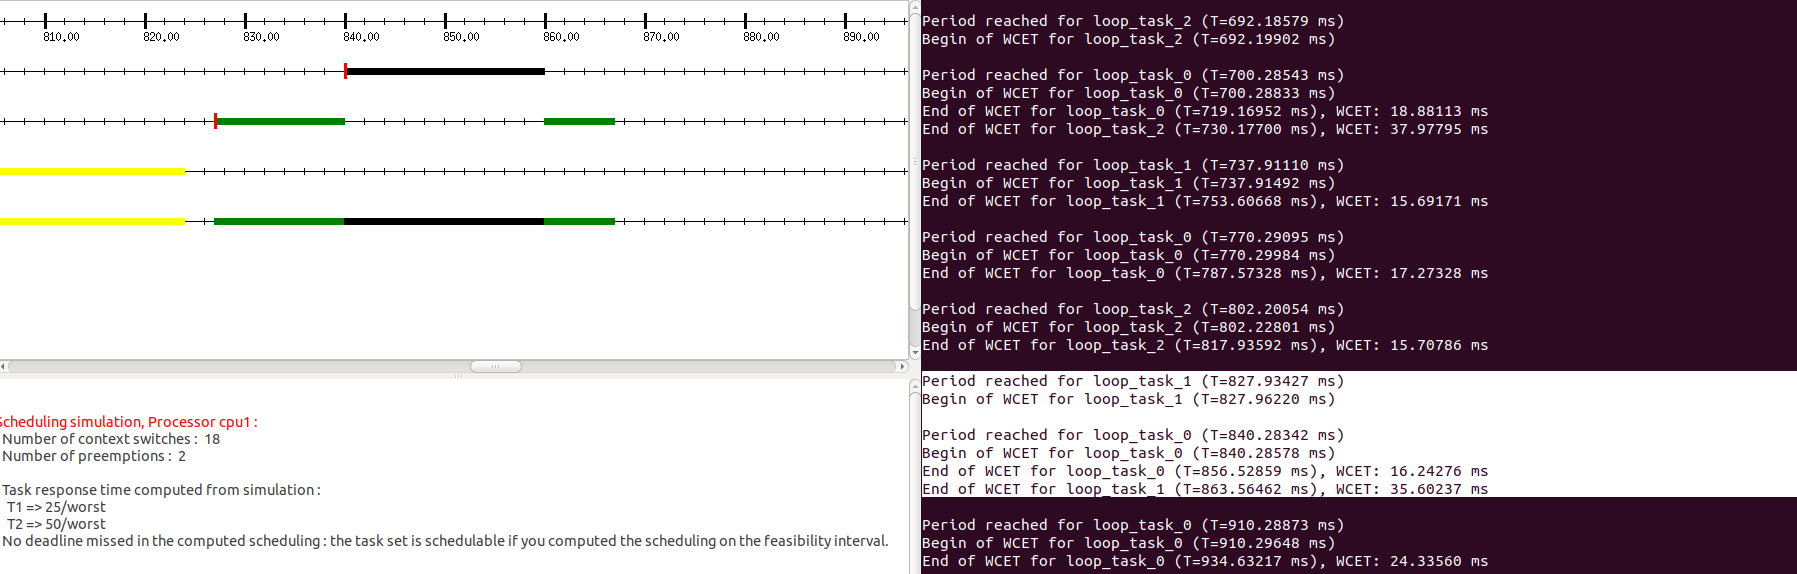
\includegraphics[scale=0.4]{T1overT2.png}
                \caption{Preemption of Task T2 by T1}
        	\end{figure} \newline
            
            \item In this second view, the task T3 is executing.At T= 700 ms , T1 which has a shortest deadline than T3 is preempted it.
            
            \begin{figure}[h]
                \hspace*{-2cm}  
                \centering
                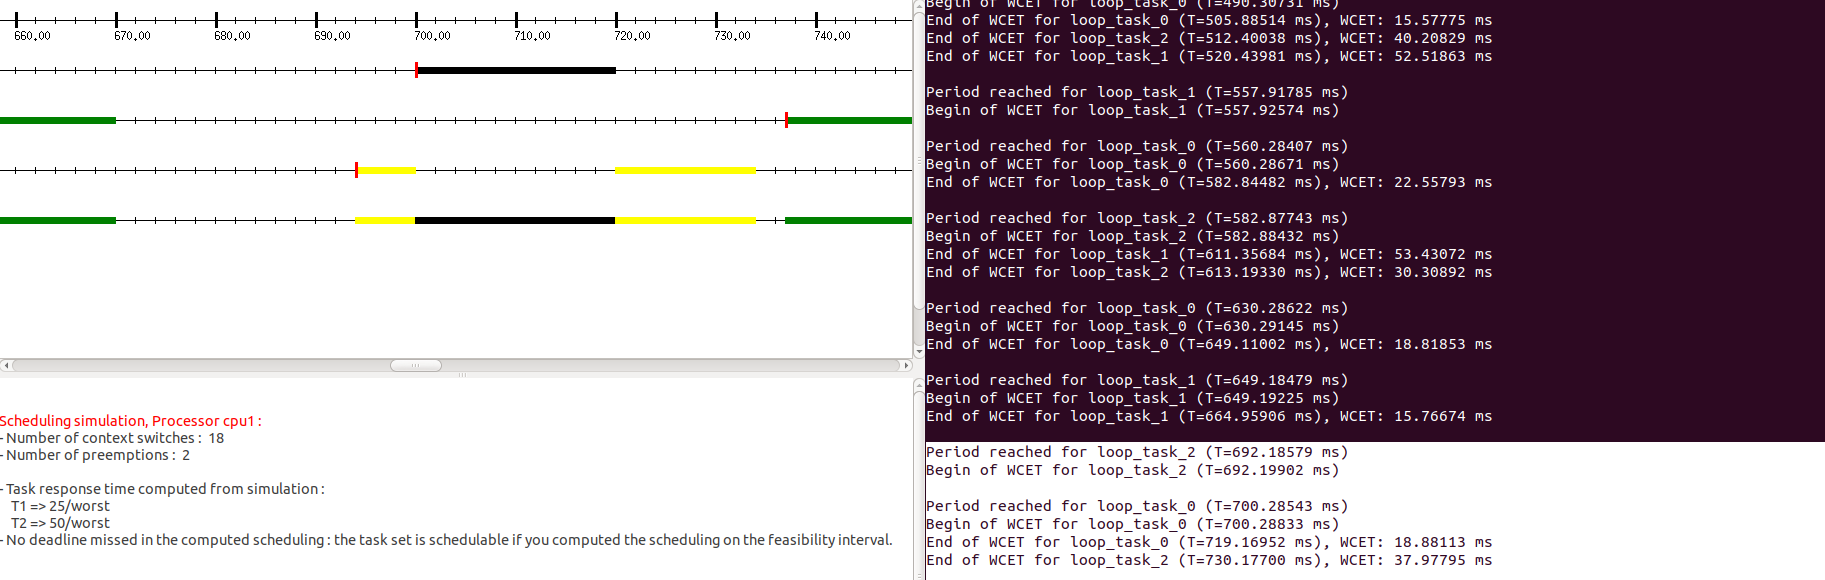
\includegraphics[scale=0.4]{T1overT3.png}
                \caption{Preemption of Task T3 by T1}
        	\end{figure} \newline
            
            \newpage \item In this last view, the task T3 is executing.At T= 384 ms , T2 which has a shortest deadline than T3 is preempted it.
         \end{itemize}           
            \begin{figure}[h]
                \hspace*{-2cm}  
                \centering
                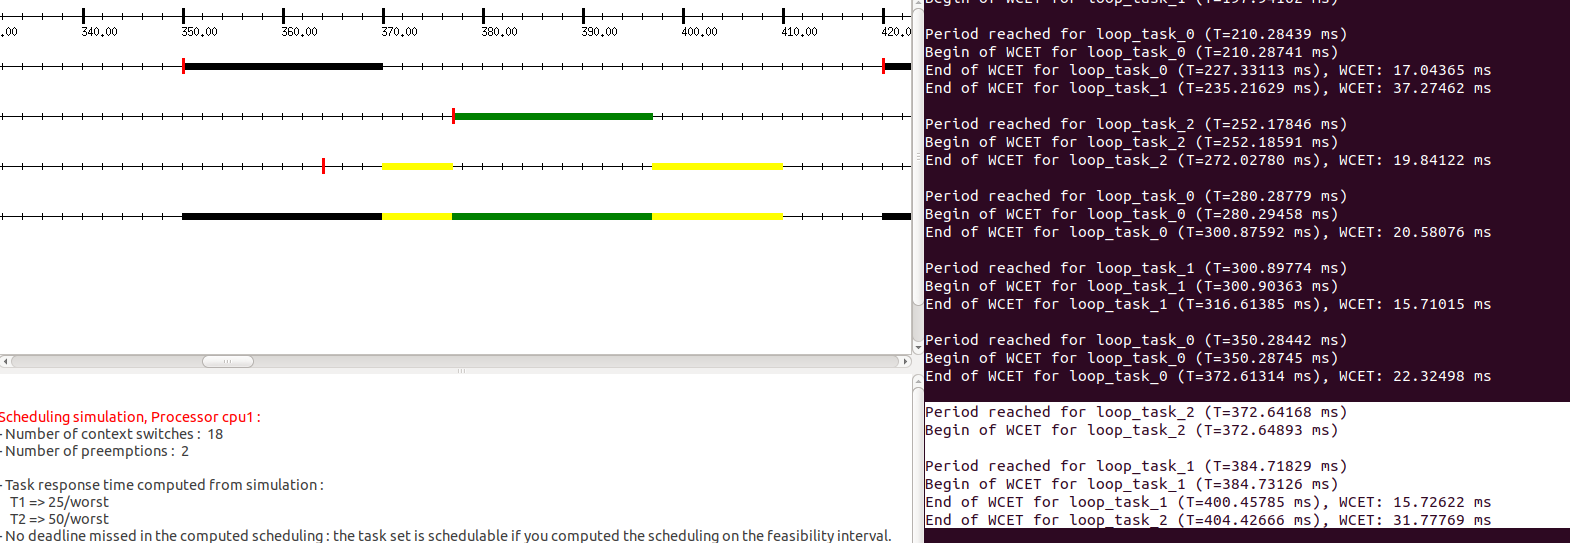
\includegraphics[scale=0.4]{T2overT3.png}
                \caption{Preemption of Task T3 by T2}
        	\end{figure} \newline
            
    Now that we have verified our EDF policy over Xenomai is working correctly, we can then have a look to the theory of ED-H policy before implementing this policy over Xenomai too.

\newpage	

\section{EH Scheduling Algorithms}
\vspace{4cm}

\subsection{Introduction}
\\Since decades batteries are accustomed store energy and providing the necessary power source for mobile, embedded and the remote system application.The development of battery techniques doesn't follow Moore's law . There are constraints like physical size,limited electric quantity, high cost etc. Restrict the performance of application like embedded systems, wireless sensor networks and low power electronics.\newline

\\There exists ambient number of energy sources from environment (tidal,solar , windmill , etc. ) which may be harvested and convert them into electric sources and It can be be later used to power wireless systems, this is often defined as energy harvesting or energy scavenging\cite{mipi-csi}.\newline

\\Energy harvesting embedded systems has been emerged as a significant topic within the field of research.There has been many research to style embedded systems which might efficiently harvest energy. The core objective of designing such systems is just to make embedded systems optimally with the available energy source.The systems are implemented in such the way that managing the power to perform operation supported current energy unit stored within the storage unit/battery and may predict the incoming energy in the future.
\begin{figure}[htp]
    \centering
    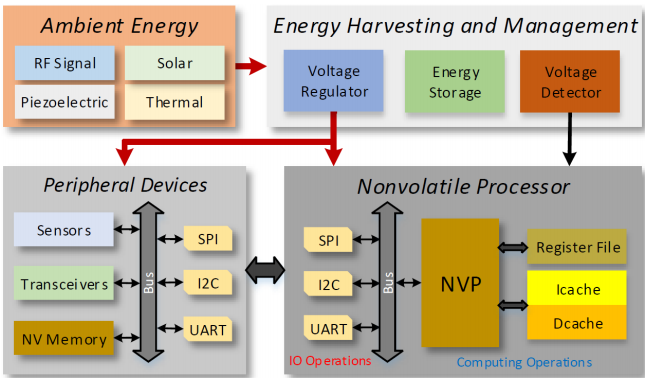
\includegraphics[width=0.7\linewidth]{Energy harvesting and managment.png}
    \caption{Architecture of Energy Harvesting Powered Sensing System}\cite{second}
    \label{fig:Architecture of Energy Harvesting Powered Sensing System}
\end{figure}
Below Figure depicts how energy is harvested from renewable environment sources.The harvested energy is regulated by energy management module to power processors and multiple peripherals.The peripheral devices consists of includes sensors,transceivers. Sensors collect the data from environment such to temperature, humidity from the environment and transceivers transmits the collected data to server for further computation.

\subsection{Energy storage systems}

\subsubsection{Battery-Related Concepts}
\newline
\\ The battery is a main power source from which energy is consumed in application mobile, portable applications thus battery capacity limits the performance.The production of current in a very given time is termed as capacity of the battery. The capacity within the battery is expressed in ampere-hours (Ah) or milliampere -hours (mAh ) \cite{battery}.\newline

There are various parameters that affect the capacity of battery like cell constructions period of time,charge and discharge cycles.The battery's capacity is approximately constant under normal operation condition during its lifetime. The lifetime of battery is reduced after they are charged incorrectly, hence they should be charged only under suitable conditions with correct charge current.To deplete the battery completely so recharge it's an acceptable method to extend the lifetime of battery.
\subsubsection{Energy Production Model}
\newline
Energy harvester unit  (eg.solar panel) produces energy from ambient renewable environment sources and converts it into electrical power at each time \textit{(t)} which later is used in embedded systems.As the energy produced from the source is unpredictable and not necessarily a constant value , we can still predict the availability in a short term perspective with worst case changing rate (WCCR) on the harvested source power output ,it is characterized by an instantaneous charging rate $P_p$\textit{(t)} that incorporates all the losses \cite{DPM_1}.Clearly we do not 
The energy which has been harvested over the time interval \textit{($t_1,t_2$)}is represented below in the following equation [1].
\begin{equation}
    E_p(t_1,t_2)=\int_{t_1}^{t_2}P_p (dt)
\end{equation}
The energy utilized in any unit time slot is not less than the energy produced in the same unit time-slot.Whenever at time \textit{t} a job is executed the residual capacity of energy storage is never increased.


\subsubsection{Energy Storage model}
\newline
The energy storage unit used in our systems (battery or supercapacitor) which are recharged up to a nominal capacity \textit{C},which corresponds to the maximum amount of energy units stored at that time \textit{t}. As we only use an ideal storage  unit, we neglect the amount of energy wasted in charging and discharging process.If the energy recharged in the battery \textit{C} exceeds maximum  capacity \textit{(C>$C_m_a_x$)}, then we consider the energy stored in battery in \textit{$C_max$}.The energy level in the battery is remain between two intervals 
\begin{equation}
    C= C_m_a_x-C_m_i_n
\end{equation}
$C_m_a_x$ and $C_m_i_n$ are upper and lower bounds of the storage unit and 
$C_m_i_n $ is not zero as there must reserved energy for worst case scenarios


If any task executing on the processor it consumes energy that is  drawn from the reservoir/battery.
The energy stored in the battery at time \textit{t} is denoted by \textit{E(t)}.There is no leakage of energy from the reservoir over time. If at time \textit{t} the energy units in battery is completely discharged $0 \leq E(t)<C_max$ is denoted by $E(t)\approx0$.The energy units in the battery at \textit{t=0} is fully charged ie \textit{E(0)=C}.

\newpage
%%%%%%%%%%%%%%%%%%%%%%%%%%%%%%%%%%%%%%%%%%%%%%%%%%%%%%%%%%%
\section{ED-H Scheduling algorithm}
\vspace{4cm}
\subsection{Introduction}
In this section we will discuss about ED-H scheduler.In classic EDF scheduler the processor is never let idle and job is executed as soon as possible thus utilizes all the energy stored in the reservoir while not saving for future energy needs.\newline
\\ Let us assume that task set is time feasible by EDF,the job $j_i$ of  $\tau_i$ will encounter energy starvation only from execution of $j_j$ of $\tau_j$ whose arrival time $a_j$<$a_i$ with $d_j > d_i$.Hence if the scheduler can predict the future arrival time of jobs and energy production it can help EDF to anticipate energy starvation and deadline violation.Thus in energy constrained systems, it is sometimes necessary not to execute the ready job if it will prevent execution of future arriving jobs due to time constraint or energy constraint \cite{EDH_ex}.\newline

\\ The main principle of ED-H is authorize job execution as long as there occurs no starvation in future.Hence ED-H is modified version of EDF which is solely used for energy harvesting constrained jobs.ED-H verifies the timing constraints , energy requirements as well as the replenishment rate of the storage unit for future arriving jobs.If one of these
conditions is not fulfilled, the processor has to idle so that
the storage unit recharges sufficiently \cite{EDH_ex1}.

\subsection{ED-H scheduling concepts}\newline
\paragraph{Static Analysis}
In this section we will study the ED-H concepts for understanding the feasibility of a job set with both energy and deadline constraints.\newline

\\The energy demand of $g_w(t_1,t_2)$ is defined as the total computation time of all the uncompleted task whose $a_i$ and $d_i$ lies between time interval($t_1,t_2$).
The energy demand of the jobset $\tau$ in given time interval \textit{($t_1,t_2$)} is calculated by 
\begin{equation}\label{energy Demand}
    g_w(t_1,t_2)= \sum_{t_1 \leq r_k,d_k \leq t_2} E_k
\end{equation}
\newline
The static slack energy $SSE_\tau$ on a jobset $\tau$ for the time interval ($t_1,t_2$) is calculated by 
\begin{equation}\label{Static Slack energy}
    SSE_\tau(t_1,t_2)= C+E_p(t_1,t_2)-g_w(t_1,t_2)
\end{equation}
where,$E_p(t_1,t_2)$=$\int_{t_1}^{t_2}P\_p(t)dt$ it is the amount of the energy that is produced by the source between $t_1$ and $t_2$.The energy demand $g_w$ \ref{energy Demand}.$SSE_tau(t_1,t_2)$   gives the maximum energy that could be made available within the  time  interval $(t_1,t_2)$ after executing jobs of $\tau$ with arrival time at or after $t_1$ and deadline at or before $t_2$ \cite{EDH_ex1}. 
\paragraph{Dynamic Analysis}
In this section we will discuss about dynamic slack energy $SE_\taui$ with respective to the current time $t_c$ in the schedule produced by $\tau$.\newline
Slack energy of a job $\tau$ for the current time $t_c$ is calculated by
\begin{equation}\label{Slack energy}
  SE_\taui(t_c)=E(t_c)E_p(t_c,d_i)-g_w(t_c,d_i)
\end{equation}
$SE_\taui(t_c)$ is calculated to determine the maximum energy that can be consumed between $t_c,d_i$ whilst guaranteeing that future arriving jobs at or after $t_c$ with deadline at or before $d_i$ have sufficient energy for its execution.There will occur energy starvation for job of $\tau$ if $SE_\taui(t_c)=$  and its deadline if after $d_i$ between $t_c$ and $d_i$.Thus ED-H provides clairvoyance on the jobs arrival time and energy production to predict possible energy starvation or deadline miss.\newline
\\The maximum slack energy that could be consumed by currently active jobs at $t_c$ while still guaranteeing the energy feasibility for the jobs that may preempt it in future is called preemption slack energy $PSE_\tau$
\begin{equation}\label{premption Slack energy}
    PSE_\tau= \min\limits_{t_c<r_i<d_i<d} SE_\tau_i(t_c).
\end{equation}

\newpage

\section{ED-H Simulator software}
\vspace{4cm}
\subsection{Introduction}
In this section we will discuss the core objective here is to develop a simulator software in C language for scheduling according to ED-H algorithm.Simulating the ED-H scheduling policies are studied in this project.\newline

The code is developed in C because as it provides optimized machine instruction for the given input which in result increases the embedded systems performance.Large memory is required when using high-level languages, when compared to high level languages we can directly control the memory using pointers and perform various process with them.We can dynamically allocate the memory, based on how much memory is required.Hence we found optimal to develop the software in C.


\subsection{Simulator structure}
The simulator software is divided in four parts. 
\begin{itemize}
    \item The first part consists of receiving the data  inputs of the task set \textbf{(T)} from the user.
    \item The second part is defined by analyzing all the feasibility checks based on ED-H algorithm.
    \item The third part comprises of scheduling the task based on the input from the user according to the ED-H algorithm.
    \item The final part is output displaying the scheduling gantt chart.
    \end{itemize}

\subsection{Simulator Packages}
The simulator consists of three main packages 
\begin{itemize}
    \item EDH.c\newline
     In this file we check the feasibility of the schedule  based upon static slack energy \textit{(SSE)} and static slack time \textit{(SST)}.Also the scheduling of the task according the ED-H algorithm is achieved from the functions defined in this file.
     \item Task.c\newline
     Here the parameters from the user are received  for each task, that is passed to task struct which is defined in this file.
     \item Schedule$\_$trace.c \newline
     In the file we display the gantt chart produced by the simulator.
\end{itemize}

\subsection{Simulator Algorithm}

The simulator software comprises of two algorithm structures.
\begin{itemize}
    \item First algorithm checks if the taskset \textbf{T} is feasible i.e static slack energy \textit{(SSE$\geq$ 0)} and \textit{(SST$\geq$ 0)}.If  the taskset \textbf{T} is feasible the simulation proceeds to schedule the with the second algorithm ,else  the simulation is terminated.
    \item Once the taskset \textbf{T} is feasible the scheduler is called to simulate the tasks. The scheduler is implemented using state machine logic and the simulation is carried out each time interval checking the energy requirements of the scheduler.
\end{itemize}
\subsubsection{Simulator Functions}

\paragraph{Feasibility Checks}\hfill
\newline

As mentioned in the earlier section the the simulator algorithm is differentiated in two parts. In this first part will discuss about the function generate$\_$ftable() which calculates  the feasibility test of the taskset \textbf{T} that is defined in EDH.c file. Once the hyper period is calculated from all the periods \textbf{($P_i$)} in the LCM() function, we pass on the  tasks {$\tau_i$} deadline {$di$} and arrival time  {$a_i$}  to  the function generate$\_$ftable().\newline

After the deadline {$d_i$} and arrival {$a_i$} time is passed, we need to calculate the processor demand \textit{$h_w$} and energy demand \textit{$g_w$} between each release time and each deadline time of every task {$\tau_i$} in the taskset  \textbf{T}.

\begin{itemize}
    \item The processor demand \textit{$h_w$} is calculated by summation of the computation time of all the task between the earliest arrival time {$a_i$} and deadline {$d_i$} (\ref{Processor Demand}).
    \item The energy demand \textit{$g_w$} is calculated by summation of the energy consumption of all the task between the earliest arrival time {$a_i$} and deadline {$d_i$}.
\end{itemize}

Next arrival times of tasks are compared and the earliest one is taken into consideration to calculate the 
the processor demand \textit{$h_w$} and energy demand \textit{$g_w$} till the deadline of each task, be it {$\tau_i$} or {$\tau_j$}.

\\ \\For instance, if the earliest arrival time were to be 0, then it would loop as such: 0-$d_i$,0-$d_j$ 0-$d_i+_1$,0-$d_j+_1$,... till 0-hyperperiod.

\\Following that, the earliest arrival time will update to the next earliest arrival time possible e.g. $T_{i,nextarrival}$

where $T_{i,nextarrival}$ = $a_i$ + $p_i$.\newline

We set to two flags $pending\_next\_arrive$ and $pending\_same\_arrive$ to true to check if processor demand \textit{$h_w$} and energy demand \textit{$g_w$} have already been calculated or not for current arrival time \textbf{$a_i$}.The flags are set in order to check if two or more task have either have same arrival time {$a_i$} or deadline {$d_i$} , so that the processor demand \textit{$h_w$} and energy demand \textit{$g_w$} are not calculated twice for same time interval. \newline

\\$pending\_next\_arrive$ is FALSE when the earliest next arrival exceeds hyperperiod, so loop can be exited and feasibility test can be terminated.\\

\\$pending\_same\_arrive$  is FALSE when all possibilities for that arrival time have been checked - i.e. for $next_{ar} = 0$, after 0-6,0-8.....0-24 (hyperperiod), no need to check again for $next_{ar}$ = 0; $next_{ar}$ can be incremented by that task's period to start next round of checking e.g. 6-8, 6-12,....6-24.\\

\\This also ensures that the arrival time is not checked twice if the next task has same arrival time as first.\\

\\Subsequently once we obtain earliest arrival time of task {$\tau_i$} from the task set \textbf{T} we need to calculate the \textit{$h_w$} and \textit{$g_w$} till the deadlines {$d_i$} of each task {$\tau_i$} in the \textbf{T}.\\


After we acquire the time intervals $t_1 $ and $ t_2$ we pass the value to $calculate\_line()$ function and  calculate the  processor demand \textit{$h_w$} and energy demand \textit{$g_w$}  of all the tasks who's arrival time {$a_i$} and deadline {$d_i$} lies between this time interval $t_1$ and $t_2$.After the \textit{$h_w$} \textit{$g_w$} is calculated we can use it find out static slack energy \textit{(SSE)} and static slack time \textit{(SST)} in the function $calculate\_line()$.\newline

The computation is repeated till we receive the all the time intervals$t_1 and t_2$. The $pending\_same\_arrive$ flag is set to FALSE after we receive all the computation for \textit{$h_w$} and \textit{$g_w$} from time $t_1$ which is the latest arrival time {$a_i$} till the deadline {$d_i$} and {$d_j$} of each task in the taskset. Then we update the $pending\_next\_arrive$ to compute the values from next arrival time of task {$\tau_i_+_1$}\\ 


If either of \textit{(SSE$\geq$ 0)} and \textit{(SST$\geq$ 0)} this two conditions is not satisfied we exit the simulation process.Once the ED-H feasibility test are passed, We calculate the sufficient schedulability condition and energy feasibility condition in the feasibilityChecks() function. If any of these three tests doesn't pass the simulation process is terminated.

\begin{algorithm}[H]
 \SetKwProg{Function}{function}{}{}
  \Function{generate-ftable}{}\\{
    \For {each task} 
    {$Task[i].next_{arrival} \gets Task[i].arrival\\
    Task[i].next_{deadline} \gets Task[i].deadline$}
    \textbf{Bool} pending-next-arrive,pending-same-arrive = TRUE 
    
    \While{pending-next-arrive}{
    \If {Task[i].next_{arrival} \geq Hyperperiod}{
    \State pending-next-arrive = FALSE}
    
    \While{pending-same-arrive}{
    endIndex \gets \Call{find-min-end}{}\\
    StartIndex \gets \Call{find-min-start}{}\\
    Earliestarr \gets Task[StartIndex].next_{arrival}\\
    Earliestdeadline \gets Task[endIndex].next_{deadline}\\
  
    \If {Earliestdeadline \leq Hyperperiod}
    {\Call{Feasibility-check}{Earliestarr,Earliestdeadline}
    }
    \If {Earliestdeadline \geq Hyperperiod}{
    pending-same-arrive = FALSE
    }\
    }
   Task[StartIndex].next_{arrival} += Task[StartIndex].period\\
  }\
 }
\end{algorithm}


\begin{algorithm}[H]
 \SetKwProg{Function}{function}{}{}
   \Function{Feasibility-check (Earliestarr, Earliestdeadline)}\\{
Calculate $hw,gw,SSE,SST_W$\\
\If {$SSE < 0$ or $SST_W < 0$\\}{
\textbf{Bool} feasibility-pass = false;\\}
\Return feasibility-pass\\}

\end{algorithm}
\newpage
\paragraph{ED-H Scheduler}\hfill
\newline


Once the taskset \textbf{T} has passed all the feasibility conditions and tests, the simulation process enters the second part where the simulator schedules according to the ED-H algorithm.The simulation process for the scheduling is developed using state machine.\newline
State machine logic was optimal for task scheduling as we need take note of different parameters - energy consumption of the task  {$\tau_i$} , slack energy \textit{(SE)} and, slack time  \textit{(ST)} are calculated for each time interval \textit{$t$} over the hyperperiod.\newline \\
There are total six states used in the simulator: 
\begin{itemize}
    \item WAITING
    \item CHECK$\_$ENERGY
    \item CHECK$\_$SLACK$\_$ENERGY
    \item CHECK$\_$SLACK$\_$TIME
    \item EXECUTE$\_$JOB
    \item EXECUTE$\_$CYCLE$\_$BY$\_$CYCLE
\end{itemize}

\begin{center}
    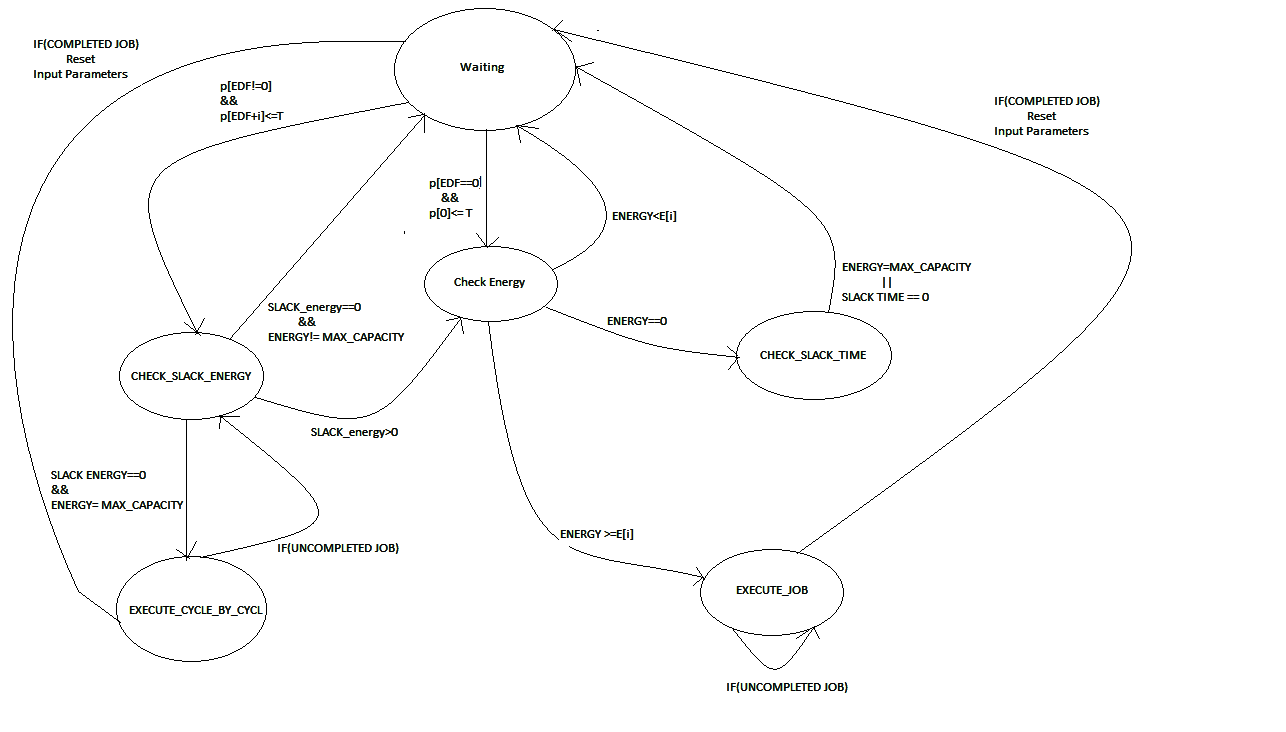
\includegraphics[width=1.0\linewidth]{CODE_STATE_MACHINE (2).png}
\end{center}

\subparagraph{WAITING}\hfill
\newline

This state is the one that is executed first when the execution starts after checking the feasibility test.In this state, sort() function is called and we pass the tasks' deadlines as input parameters to set the priority of the tasks {$\tau$} according to earliest deadline first. The highest priority task is stored in the $0^{th}$ position in run-queue.\newline

Next, within the waiting state itself, scheduling too happens. The scheduler can necessarily only schedule tasks that are released before or at the current time \textit{$t_c$}, known as eligible tasks.\\

To begin, if the highest-priority task {$\tau_0$} is eligible, the processor switches to the CHECK$\_$ENERGY state to check if the energy \textit{E} in battery is sufficient for execution of task $\tau_i$\newline.

However, if {$\tau_0$} is not eligible, the next highest priority task {$\tau_1$} is checked for eligibility and if that too is not, then {$\tau_2$} and so on. In this way, it goes down the priority list until it finds an eligible task. Since this task is not of highest priority, unlike {$\tau_0$}, and there is a possibility of pre-emption by a higher priority task in future, processor instead enters CHECK$\_$SLACK$\_$ENERGY state, where it is checked if slack energy is sufficient to authorize the task.\newline

If there is no task ready in the run-queue the scheduler goes to idle state and battery is recharged till the next arrival time {$a_i$} of task in the run-queue.

\begin{algorithm}[H]
\DontPrintSemicolon
  \KwInput{Tasks ($\tau_0$ to $\tau_{fin}$) and their arrival times $t_{arr}$, current time $t_c$}
  \KwOutput{Tasks sorted by priority for energy state checking}
  \KwData{prioritylist}
  EDF = 0 \tcp*{initialize counter}
  \tcc{Prioritizing tasks by earliest deadlines}
   prioritylist \gets \Call{Sort}(Tasks)
  
  \If{prioritylist[0].$t_{arr}$ $<$ $t_c$}{
  case $CHECK$ $ENERGY$\ $state$;}
  
  \Else 
         {\For{EDF \in [1,fin]}    
        {
        	\If {prioritylist[EDF].$t_{arr}$ $<$ $t_c$}
        	{case CHECK SLACK ENERGY state;\\
        	break;}
        	\If {EDF == fin}
        	{No task found;\\
        	Enter idle period for recharging cycle;\\
        	break;}
        	EDF++;\\
        }
    }
\caption{WAITING State}
\end{algorithm}

\newline
\subparagraph{CHECK$\_$ENERGY}\hfill \label{SlackMethodEnergy}
\newline

After the task has been selected from the run-queue, the scheduler enters the CHECK$\_$ENERGY state. Here, the energy units \textit{E} in the battery are checked to see if they are sufficient to execute the task which is currently ready. If the energy in battery is completely depleted \textit{(E==0)}, the processor cannot execute tasks – so we need to introduce an idle period during which the battery can recharge, known as the  recharge cycle. \\

Slack time (ST) is the maximum time the processor can be idle to avoid deadline miss (also known as time starvation). Hence, the processor needs to constantly check the slack time to see how long it can idle.\\

To begin, if ST has not yet been checked at $t_c$, it switches to CHECK$\_$SLACK$\_$TIME. However, if it has been checked and still, battery level is zero, the scheduler goes to the idle mode and charges for one time period. After this one recharge, it does CHECK$\_$SLACK$\_$TIME again to avoid any deadline miss (in case slack time is 0 at the new $t_c$ and it needs to switch to WAITING state to take in updated tasks).\\

If battery energy is non-zero \textit{(E$\neq$0)}, there is a possibility to begin a task but that is not enough - the scheduler should also verify that there will be sufficient energy to execute it completely. This brings the need for residual energy forecasting. \\\\

\textbf{2.1 Residual Energy Forecasting}\\

The amount of residual energy in the battery that will be remaining after task completion at a future time depends on both the current energy level and the percentage of the task that has already been executed (this is tracked by a boolean member variable belonging to the struct 'task', known as \textbf{ongoing}). \\

\textbf{ongoing} = 0 if the active task is yet to begin and  = 1 if it has already executed some portion.\\

The scheduler now calculates the remaining energy units \textit{E} after executing the task. If \textbf{ongoing} = 0,  residual energy in battery after job will be completed is forecast as:
\begin{equation}
\textbf{$Remaining$\_$energy=E(t)+(P_p*C_i)-e_i$}    
\end{equation}

If \textbf{ongoing} = 1,residual energy in battery after job will be completed  is forecast as:
\begin{equation}
    Remaining\_energy = E(t) + (P_p * (C_i - executed\_time)) - (e_i - consumed\_energy)
\end{equation}

where
\begin{itemize}
    \item E(t)= Energy Units in the storage unit(Battery) at time \textit{t}
    \item $P_p$=Rechargeable power constant over the hyper-period
    \item $C_i$= Computation time of task $\tau_i$
    \item $executed\_time$= Already executed time of task $\tau_i$
    \item $e_i$= Total energy consumption of task start to end $\tau_i$
    \item $consumed\_energy$= Already consumed energy of task $\tau_i$ corresponding to its residual computation time.
\end{itemize}

Maximum possible battery energy is capped off at Emax.\\

In the following two cases:\\
\begin{itemize}
    \item If remaining energy is forecasted to be $<$ 0 i.e. energy starvation is detected
    \item If initial energy available is not enough to even execute the task for one computation time.\\
    \end{itemize}
    
The processor introduces idle time to recharge the battery for one time period before switching state to WAITING, so that processor can assign an updated schedule based on updated task deadlines (and hence, priorities) and arrival times.\\

If the available energy is sufficient for executing the job, case EXECUTE JOB commences, where the scheduler executes the ready task $\tau_i$.\\

\begin{algorithm}[H]
\SetAlgoLined
\DontPrintSemicolon
  \KwInput{Energy in battery (E),E_{max}, Active Job ($\tau_i$), Recharge-rate($P_p$), \bool SlackChecked, current time$(t_c)$}
  \KwOutput{Residual Energy after Job Completion, E_{residual}}
  \textbf{For each job: }{Computation time $C_i$, already executed time $t_{Ei}$, total energy $e_i$, already consumed energy $E_{ci}$, bool ongoing}
  
  \tcc{Checking if battery energy is enough to execute task, or if it needs recharge}
  
  \If{E == 0}{
    \tcc{Idle time is needed for recharge; maximum allowable idle time is calculated by checking SLACK\_TIME}
      \If{SlackChecked == TRUE \tcp*{Checking if SLACK\_TIME has been checked since t=0}}
        {\If{SlackCheckedTime == t \tcp*{Check if SLACK\_TIME's checked at t_c}}{
            {Recharge by $p_p$ for one time-period and update $t_c$}
        }
        {state = CHECK\_SLACK\_TIME} \tcp*{Check SLACK\_TIME at $t_c$}
        {break \tcp*{exit CHECK\_ENERGY once CHECK\_SLACK\_TIME is called\}}
    }}\\}
    
    \eIf{{$\tau_i$.ongoing} == 0 \tcp*{ongoing = 0 means active task has not begun}}{
       E_{residual} = E + (P_p * C_i)-e_{i}\\}
      {\tcc{ongoing $\neq$ 0 means active task has begun} E_{residual} = E + (P_p * (C_i - t_{Ei}))-(e_{i}-E_{ci})\\}
    
    \eIf{$E_{residual}$ is sufficient}{state = EXECUTE\_JOB}{Recharge for one time period.\\state = WAITING\\}

\caption{CHECK\_ENERGY State}
\end{algorithm}

\subparagraph{CHECK$\_$SLACK$\_$TIME}\hfill \label{SlackMethodTime}
\newline

To recall from the previous section, the processor enters the CHECK$\_$SLACK$\_$TIME state from CHECK$\_$ENERGY state When the energy in the battery is completely depleted. It continually loops within this state until battery energy reach Emax or the scheduler cannot be idled further for recharging due to the minimum ST equating to 0.\\

Slack time (\textit{ST}) can be defined as the maximum time the scheduler can be idled for recharging and the active task can be delayed without causing deadline miss of other tasks in the taskset. It is calculated via the following steps: \newline


The variable \textit{minSlack}, which stores the shortest ST among all tasks, is updated with the newly calculated ST if this ST $<$ \textit{minSlack}.\\

Either if energy in battery has reached its max capacity or the calculated Slack time \textit{ST} results to 0, the processor cannot be idled for any further time period and the scheduler enters $WAITING$ state.
\newline


\begin{algorithm}[H]
\DontPrintSemicolon
  \KwInput{Each task $\tau_i$, each job $J_k$, Release times of the task $r_i$, release time of job is $r_k$ , Partially completed jobs remaining computation time is $C_{k,rem}$ , job not yet released has computation time $C_k$ and deadline of job is $d_k$ , deadline of task is $d_i$ , current time $t_c$}
  \KwOutput{ST for each job of task $\tau_i$ }
  \
  \For {All Jobs in task\ $\tau_i$ at time t_c}
    
    \If{(C_{k,rem} != 0) \And  (d_k \leq d_i) \tcp* {If job is incomplete}}{C_{tot,rem} += C_{k,rem} \hspace {3}} 
    
    \If{(t_c <= r_k  \And  d_k <= d_i) \tcp* {If the job will be released in future (t_c <= $r_k$)}}{C_{tot,fut} += C_{k}}
{{ST_{$\tau_i$} = d_i - t_c − -C_{tot,rem}$ - $C_{tot,fut}$}}
\caption{CHECK\_SLACK\_TIME State}
\end{algorithm} 

\begin{algorithm}
 \tcc {Dynamic ST is the minimum slack time of all jobs ending after current time.} 

    Dynamic ST_{w} = min(all$ ST_$\tau_i$ s with $d_i$ $\geq$ $t_c$)
\end{algorithm}
\KwOutput{ST for each job of task $\tau_i$ }

\subparagraph{CHECK$\_$SLACK$\_$ENERGY}\hfill
\newline
\newline
The simulator enters this state when high priority task is forecast-ed to be released after the current time \textit{$t_c$}, in which case, it will pre-empt the running lower priority job. In this state, SE is calculated for the lower priority job to ensure there is sufficient energy to run a higher priority task in case it arrives in future.\\

\begin{algorithm}[H]
\SetAlgoLined
\DontPrintSemicolon
\KwInput{Each task $\tau_i$, each job $J_k$, Release times of the task $r_i$, release time of job is $r_k$ , Instantaneous recharging Pp, deadline of job is $d_k$ , deadline of task is $d_i$ , Energy at current time is $E(t_c)$, $e_w$ is total energy consumed by all jobs, $E_k$ is job's energy, Preemption  consumed by future job, current time $t_c$}

  \KwOutput{Slack energy {SE} for each job of task $\tau_i$ }
  
  \For {All Jobs in task\ $\tau_i$ at time $t_c$}{

    \If{($t_c$ \leq $r_k$  \And  $d_k$ \leq $d_i$) \tcc {If the job will be released in future, Add job's energy $E_k$ to $e_w$}} { e_w += E_k } } 
    
SE_{\tau_i} = E(t_c) + (d_i-t _c)*Pp - e_w
\caption{CHECK\_SLACK\_ENERGY State}
\end{algorithm} 

\begin{algorithm}
 \tcc {Dynamic preemptive SE (PSE) the minimum SE of all tasks releasing after current time and with deadline $d_i$ before $d_{max}$.} 

     Dynamic PSE_{w} = min(all$ SE_$\tau_i$ s with $d_{max}$ $\eq$ max_w(d_i)
\end{algorithm}
\newline

\subparagraph{EXECUTE$\_$JOB}\hfill
\newline

The scheduling of task $\tau_i$ is simulated in this state only if
\begin{itemize}
    \item $\tau_i$ is the highest priority task at $t_c$\\ \\
    or if it is not the highest priority task, 
    \item SE is positive and residual battery energy ${E_{res}}$ sufficiently high for $\tau_i$ to execute. 
\end{itemize}

\textbf{THE PROCESS}
\begin{enumerate}
    \item The \textit{ongoing} variable of this task $\tau_i$ is set to 1, to acknowledge that this job is about to be executed for at least one time period and is not a fresh task. 
    \item The executed time \textit{$t_{Exci}$} of job $\tau_i$ is incremented by 1 each time the state is called, till \textit{$t_{Exci}$} is equal to computation time $C_i$. We store this value to keep track of how many computation units \textit{$c_i$} have been executed.
    \item If job is incomplete, run EXECUTE JOB again
    \item Else, the job is complete, so
    \begin{enumerate}
        \item shift deadline and arrival time by one period for next execution
        \item reset \textit{ongoing} and \textit{$t_{Exci}$} to 0
        \item switch to state WAITING to execute next ready task $\tau_i_+_1$.
    \end{enumerate}
    
\end{enumerate}

\begin{algorithm}[H]
\DontPrintSemicolon
  \KwInput{Active job's $t_{Exci}, C_i, D_i, t_{arr,i}, P_i$}
  \KwOutput{Desired state}
  
   ongoing = 1 \tcp*{Indicates job has started}\\
   t_{Exci}\  += 1 \\
   \tcc{If job is unfinished at end of cycle}
   \If {t_{Exci} < C_i} 
   {State = EXECUTE\_JOB}
   
    \Else{
    \tcc{Shift arrival times and deadlines by task period.}
    t_{arr,i}\ += P_i\\ 
    D_i\ += P_i\\
    State = WAITING\\
    \tcc {Reset variables to 0}
    t_{Exci} = 0\\
    ongoing = 0\\
    }
\caption{EXECUTE\_JOB State}
\end{algorithm}

\subparagraph{EXECUTE$\_$CYCLE$\_$BY$\_$CYCLE}\hfill
\newline

This state is called from the CHECK$\_$SLACK$\_$ENERGY state, specifically when the slack energy is $\leq$ 0 while $E=E_{max}$. Recall that CHECK$\_$SLACK$\_$ENERGY is first called when a higher priority task is forecasted to arrive after the current time \textit{$t_c$}, such that it will preempt the low priority active task $\tau_i$.\\

\textbf{THE PROCESS}
\newline
In this state, along with the variables \textit{ongoing} and \textit{$t_{Exci}$} as defined in the state EXECUTE$\_$JOB, we introduce a new variable \textit{$E_{used,i}$} to keep a track on how many energy units \textit{$e_i$} have been consumed by a job up to pre-emption.

\begin{enumerate}
    \item  $E_{used,i}$ is the energy consumed by task $\tau_i$ after executing some amount of computation time. It is calculated as: 
    
    \begin{equation}
            E_{used,i} += (e_i / C_i) 
        \end{equation}
        
        where
        
    \item Next, the residual energy in battery after the $\tau_i$ is executed for one cycle is calculated as 
         \begin{equation}
            E = E - (e_i / C_i) + P_p
        \end{equation}
    \item If job is unfinished at the end of the cycle, it enters the CHECK$\_$SLACK$\_$ENERGY state again to check if
    \begin{itemize}
        \item \textbf{SE $>$ 0 \And $E=E_{max}$:} it can move to CHECK\_ENERGY then EXECUTE\_JOB or
        \item \textbf{SE = 0 \& $E=E_{max}$} it needs to continue executing cycle by cycle 
        or 
        \item \textbf{SE\ !=$E_{max}$}: It needs recharge.
    \end{itemize}
    
    \item Else, it means that the job is complete, so 
        \begin{enumerate}
            \item shift deadline and arrival time by one period for next execution
            \item reset \textit{ongoing}, \textit{$E_{used,i}$} and \textit{$t_{Exci}$} to 0
            \item switch to state WAITING to execute next ready task $\tau_i_+_1$.
        \end{enumerate}
\end{enumerate}

\begin{algorithm}[H]
\DontPrintSemicolon
  \KwInput{Active job's $t_{Exci}, C_i, D_i, t_{arr,i}, P_i$, $E_used,i$, $e_i$, $P_p$}
  \KwOutput{Desired state}
  
   ongoing = 1 \tcp*{Indicates job has started}\\
   t_{Exci}\  += 1 \\
   \tcc{Increment energy used by per-cycle-energy consumption of task} 
   E_{used,i}\ += 1 \\
   \tcc{If job is unfinished at end of cycle}
   \If {t_{Exci} < C_i\\ 
   \tcc{To check values of SE and E}}
   {State = CHECK\_SLACK\_ENERGY} 
   
    \Else{
    \tcc{Shift arrival times and deadlines by task period.}
    t_{arr,i}\ += P_i\\ 
    D_i\ += P_i\\
    State = WAITING\\
    \tcc {Reset variables to 0}
    t_{Exci} = 0\\
    ongoing = 0\\
    }
\caption{EXECUTE\_CYCLE\_BY\_CYCLE State}
\end{algorithm}
\newpage
%%%%%%%%%%%%%%%%%%%%%%%%%%%%%%%%%%%%%%%%%%%%%%%%%%%%%%%%%%%
\section{Message pipes services}
\vspace{4cm}
 %https://www.programmerall.com/article/46162171901/
	As explained in the previous section, ED-H policy required to have battery information.More particularly, we need the battery capacity and also the energy produced for a given interval in order to compute slack\_energy of each task each time the scheduler is called.
	
	However we are using a dual-kernel configuration, I mean Xenomai Real Time tasks are running on the \textbf{Cobalt} kernel while non-real time tasks are running on the default Linux kernel.
	
	We will have so :
	\begin{itemize}
	    \item Several real-time tasks : tasks scheduled with ED-H policy + the scheduler
	    \item A non real-time task : used to gather battery information from Linux kernel API.
	\end{itemize}
	
	In order for the scheduler to access the battery information from the non real time task, we need to find a way to establish proper communication  between real-time task and non real-time task.
	
	Few solutions exist :\begin{itemize}
	    \item XDDP communication : a native solution using communication pipe, fully supported since Xenomai 2.0
	    \item RT CAN bus or RT USART or RTnet (TCP/IP socket interface) : useful when your Cobalt is on a different board than your Linux Kernel
	    \item shared memory
	\end{itemize}
	
	Because XDDP communication is easy to deploy, we will explain and then show how to use this solution in order to retrieve battery information from a RT context.
	
	\subsection{XDDP communication : How it works}
	
    As explained before, Xenomai runs alongside the default Linux kernel. (using an Hardware abstraction layer called \textbf{adeos}). In our configuration (I mean a dual Kernel configuration), Xenomai has the higher priority and Linux the lowest. That mean each Xenomai task which use no Linux system calls or APIs within the code have a higher priority (they are in \textbf{primary mode} than other tasks using it (these tasks are in \textbf{secondary mode}).
    
    On top of that, switching from primary mode to secondary mode could lead to priority inversion problem (a higher priority task being preempted by a task with a lower priority).
    
    So to prevent all this, we need a pipe mechanism called the XDDP. This mechanism can be used directly thanks to the POSIX skin of Xenomai (I mean a subset of POSIX functions for Xenomai only, which include XDDP mechanism).
    
    \begin{figure}[ht]
    \centering
	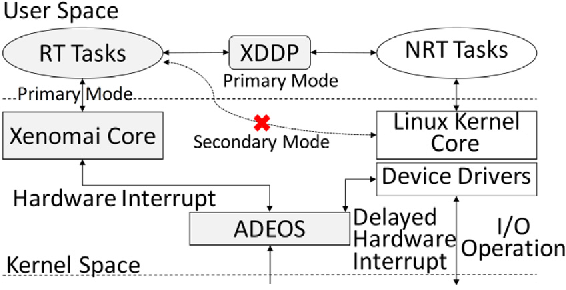
\includegraphics[scale=0.7]{SW.png}
	\caption{SW Architecture for RT-nRT  communication}
	\end{figure} \newline
    
    Basically, the XDDP mechanism use message pipes to communicate between real-time tasks and regular Linux tasks. A communication pipe could only be open by a Xenomai RT tasks.Then a non-RT task could write/read data shared on the pipe by accessing it from the Linux standard filesystem (I will explain this later).
    
    The figure below illustrates the RT - non RT communication process using XDDP :
    \begin{figure}[ht]
	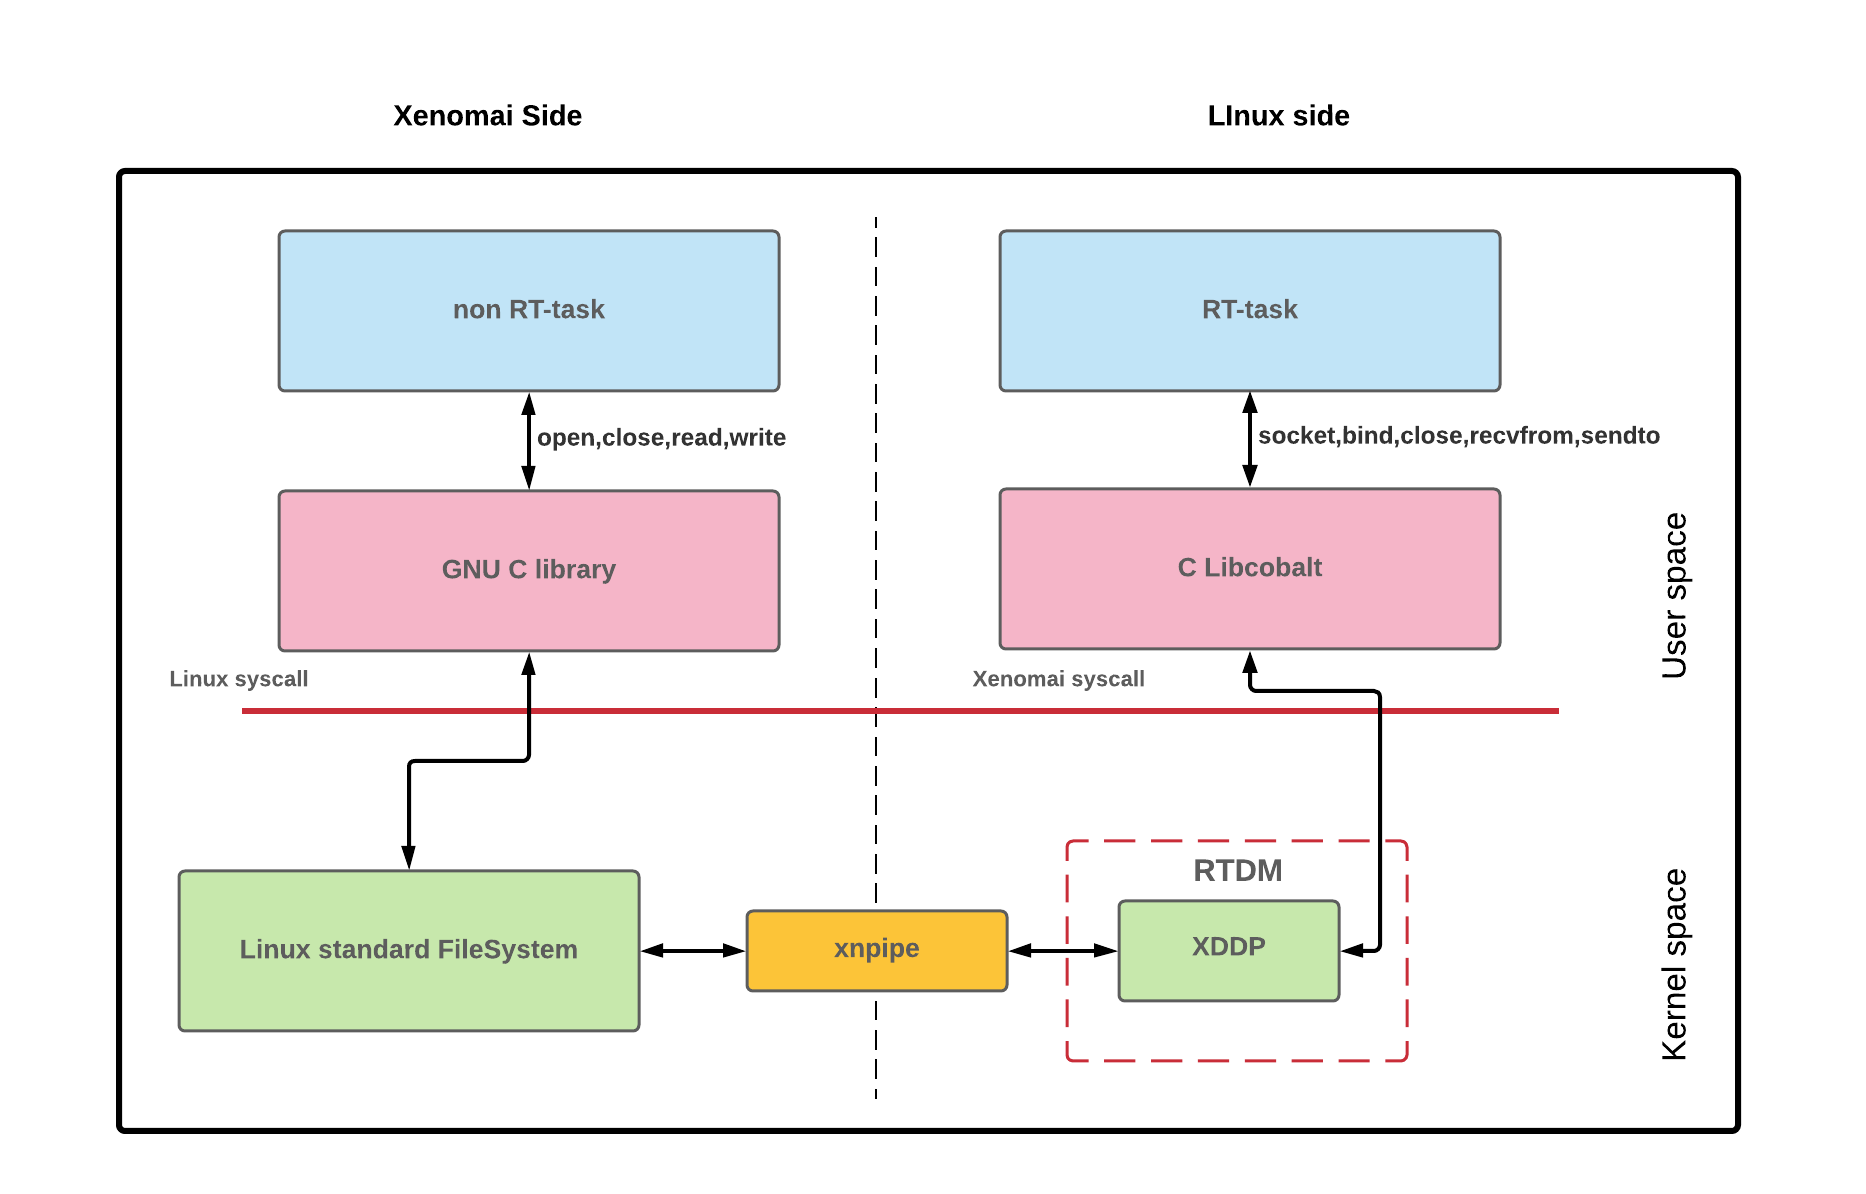
\includegraphics[scale=0.25]{XDDPcom.png}
	\caption{Simplified diagram for XDDP communication}
	\end{figure} \newline
	
	On the Linux domain side, pseudo-device files named /dev/rtp<minor> give regular POSIX tasks access to non real-time communication endpoints, via the Linux standard File System service. 
	\newline On the Xenomai domain side, a socket is bound to an XDDP port, which will then act as a proxy to send and receive data to/from the associated pseudo-device file. Keep in mind that XDDP port and minor number are the same and so :
 
 \begin{itemize}
     \item data sending through a XDDP socket using sendto() function could be received in the Linux domain via the standard read() function
     \item data receiving through a XDDP socket using recvfrom() function have been sent from the Linux domain via the standard write() function
 \end{itemize}
 
 Figure below illustrates functions call in Linux domain and Xenomai domain :
 
     \begin{figure}[ht]
    \hspace{-2cm}
	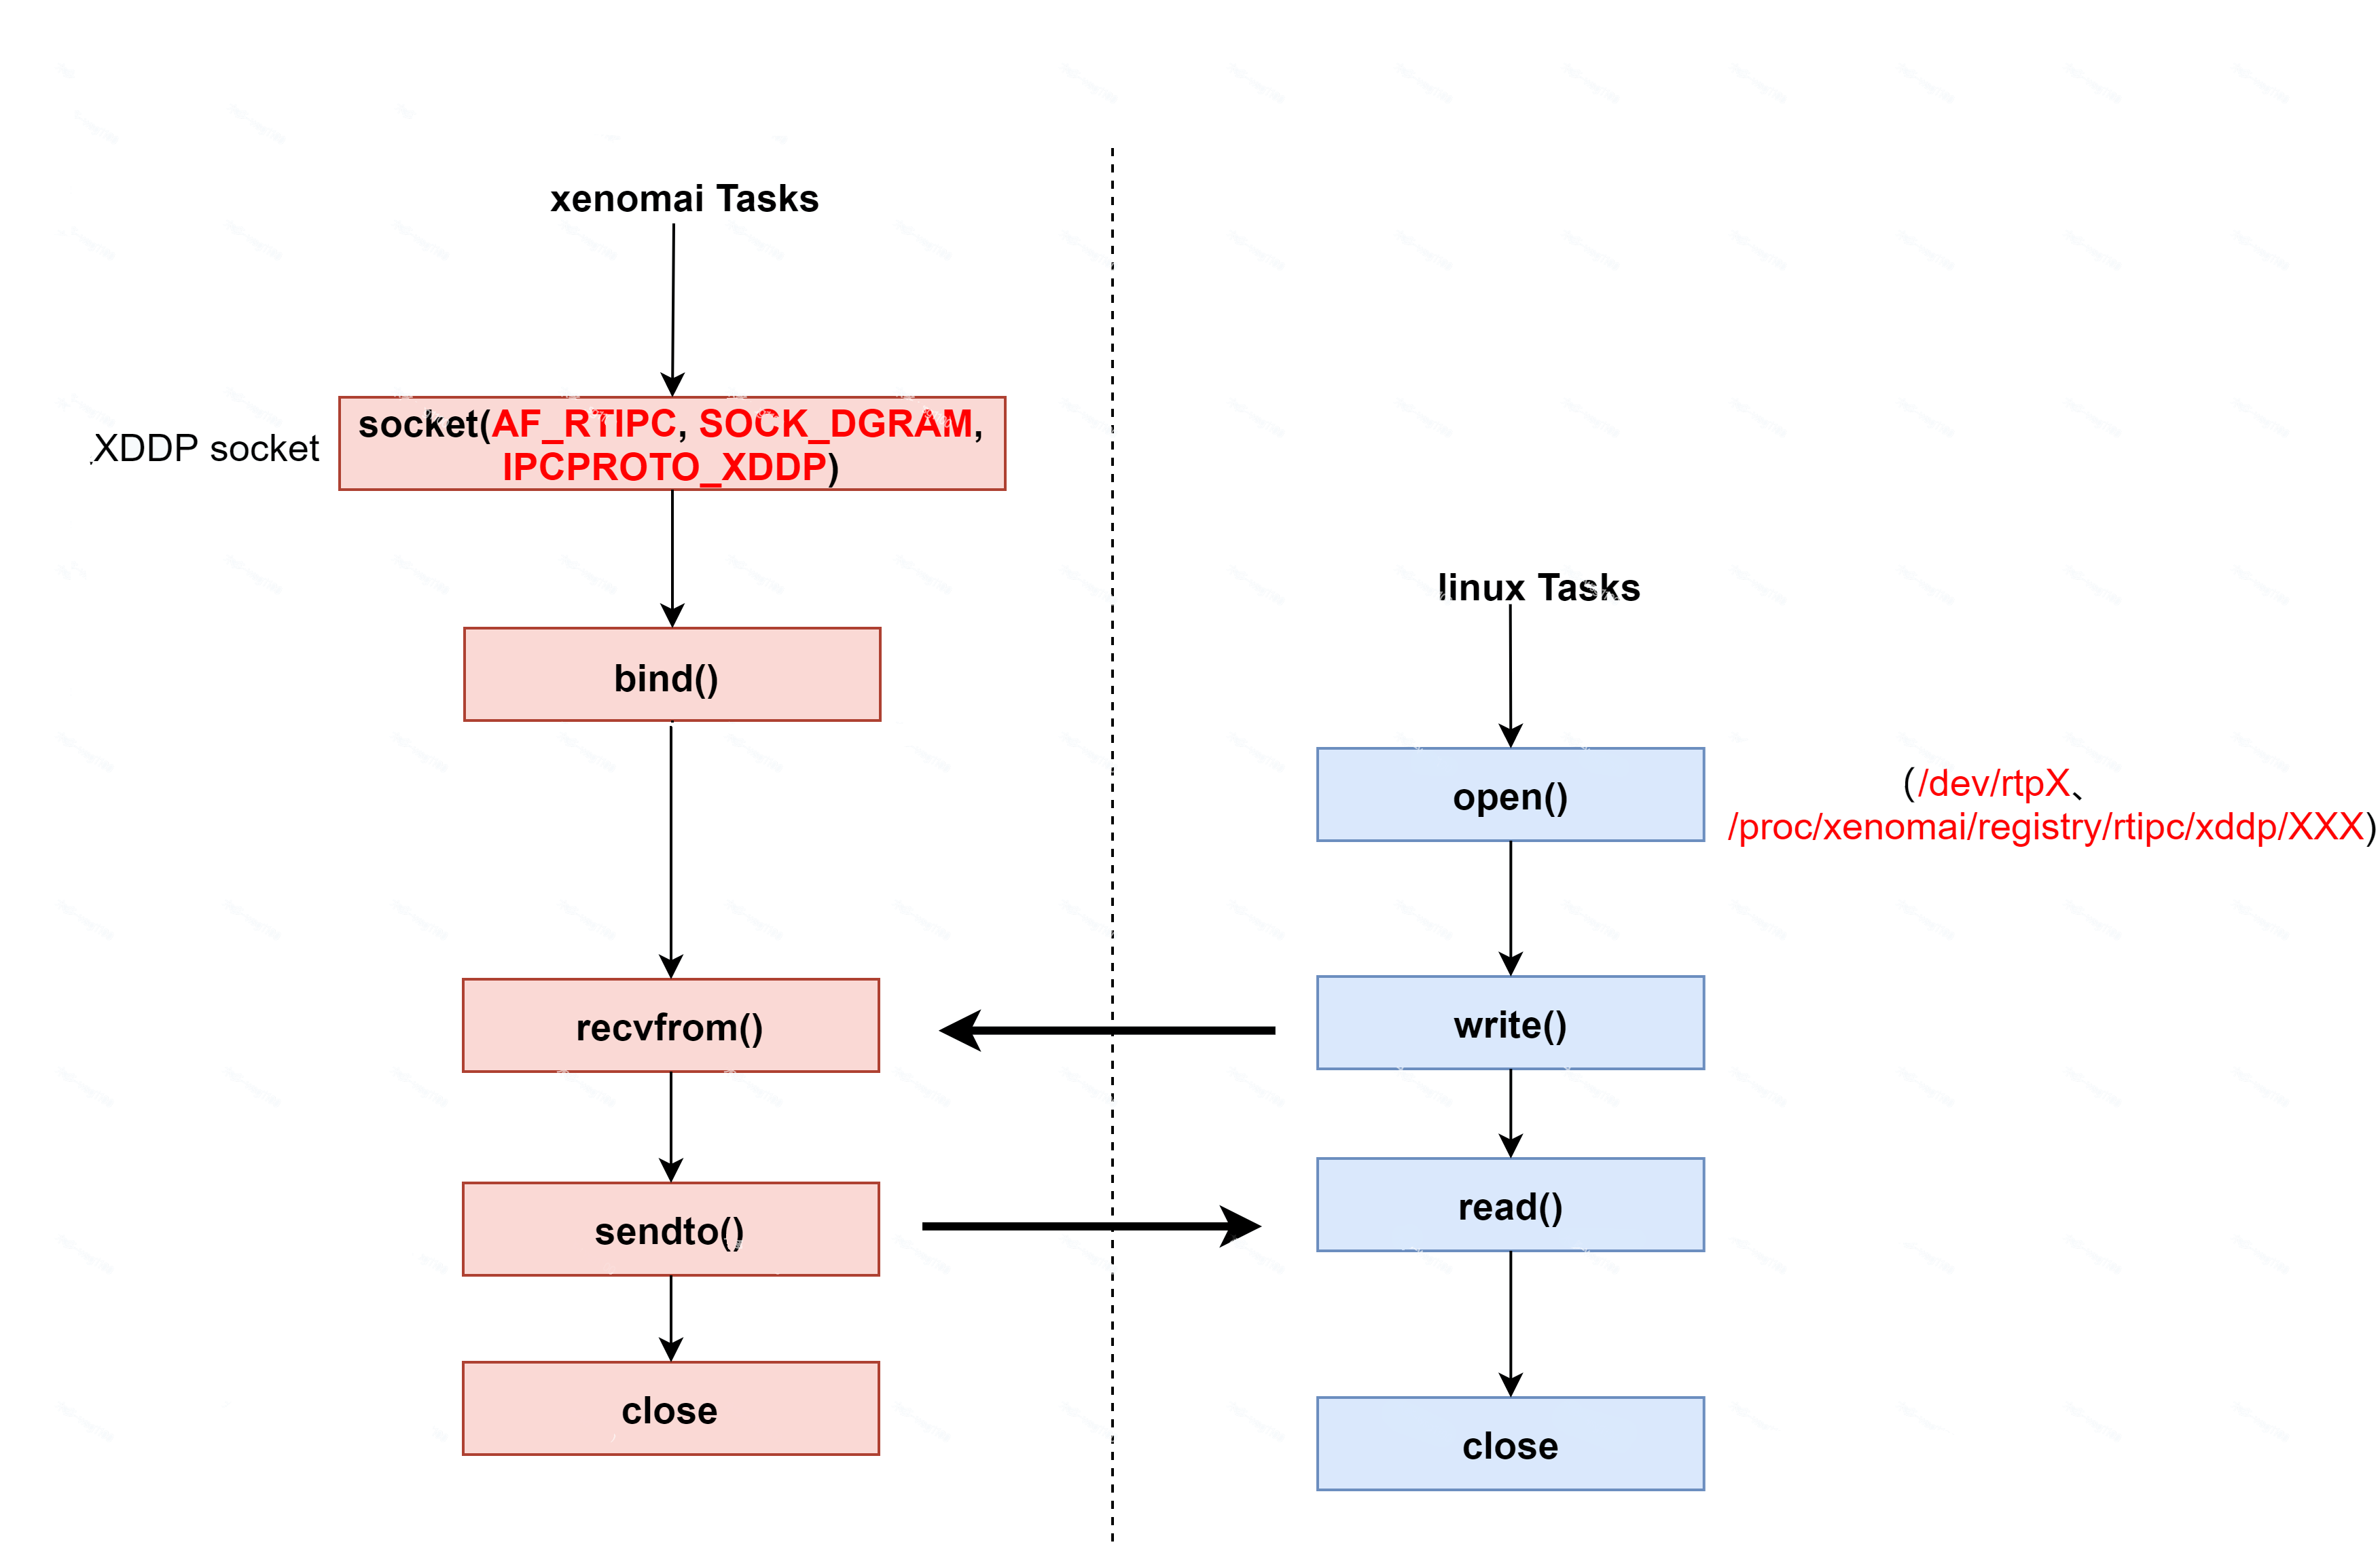
\includegraphics[scale=0.2]{XDDPhowTo.png}
	\caption{Functions call in both domains}
	\end{figure} \newline
 
 We made a simple example to show you how to bind a socket and read data from RT tasks \href{https://github.com/skyultime/M2_ERTS_Project_Xenomai_edh/tree/dev/SourceCode/xttpProtTemplate}{here}:  
 
 Another similar example, available \href{https://github.com/skyultime/M2_ERTS_Project_Xenomai_edh/tree/dev/SourceCode/XenomaiSideXddpExample}{here}, use functions with the RT\_PIPE\_ prefix. This is simply an API to simplify the whole process (indeed RT\_PIPE\_CREATE call directly the socket() function for example).\newline
 
 Xenomai also provides example which are available \href{https://Xenomai.org/documentation/Xenomai-3/html/xeno3prm/xddp-echo_8c-example.html}{here} as well...

	\subsection{XDDP communication to retrieve battery data}
    	
	As explained before, we need first a RT task dedicated to create socket and then retrieve information from the battery. Then we need a non-RT task dedicated to send battery information from the Linux domain. While the RT task can be directly the one use to schedule all Xenomai tasks (I mean we can retrieve battery information just before selecting the next thread to be executed), we need to create a Linux module dedicated to get battery information.
	
	Rather than using a simple application in user space which we can launch each time we need to use, the interest of using a module is :
	\begin{enumerate}
	    \item Inserting the module at boot (I mean the module will be automatically started during boot operation).
	    \item Easy way to load/unload the module dynamically
	    \item Direct call of kernel space functions
	\end{enumerate}
	
	The Linux battery module is available \href{https://github.com/skyultime/M2_ERTS_Project_Xenomai_edh/tree/dev/SourceCode/LinuxBattModule}{here} (with README file as well).\newline
	
	In this module, we can observe 3 main parts :
	\begin{itemize}
	    \item The init section : Basically, we use the equivalent read() function to access a socket on port 0 (=minor 0) . We also create a timer, of \textbf{TIMER\_LENGTH} ms duration. Each time the timer expires, a work task dedicated to send battery information through the XDDP port 0 will be called through the timer handler. (cf. \href{https://Linux-kernel-labs.github.io/refs/heads/master/labs/deferred_work.html}{here} to understand the basis of workqueue and deferred work).
	    
         \begin{figure}[ht]
         \centering
    	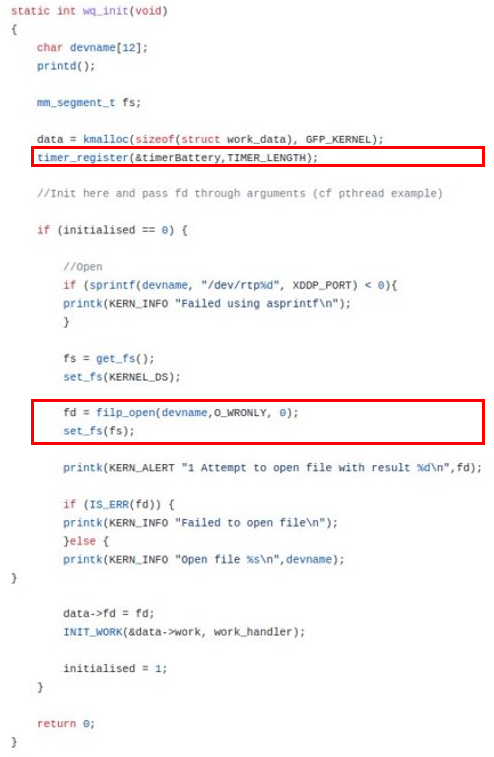
\includegraphics[scale=0.6]{init.png}
    	\caption{Init section for battery Linux module}
    	\end{figure} \newline
	    
	    \item the timer handler : Each time the timer expires, he will call the work task.
	    
         \begin{figure}[ht]
         \centering
    	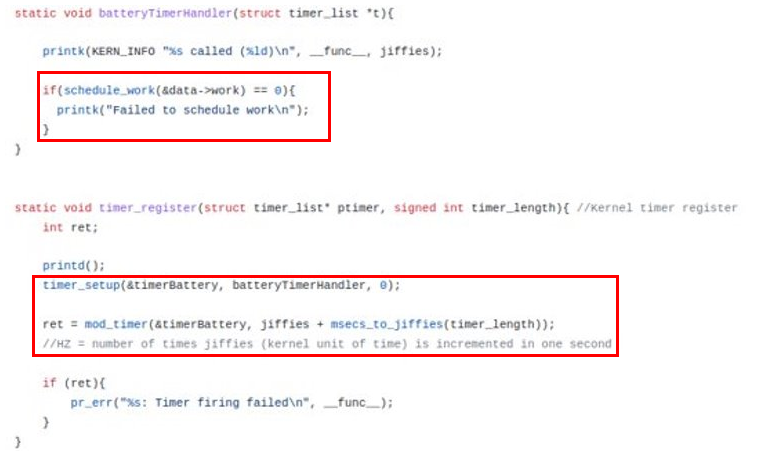
\includegraphics[scale=0.6]{timHandler.png}
    	\caption{Time handler for battery Linux module}
    	\end{figure}
	    
	    \newpage \item the work task : Gather battery information via \textbf {\href{https://www.kernel.org/doc/html/latest/power/power_supply_class.html}{<Linux/power\_supply>}} and send it via standard write() function. Once all operations are operated, the work task relaunch the timer.\newline
	  
	    \begin{figure}[!h]
         \centering
    	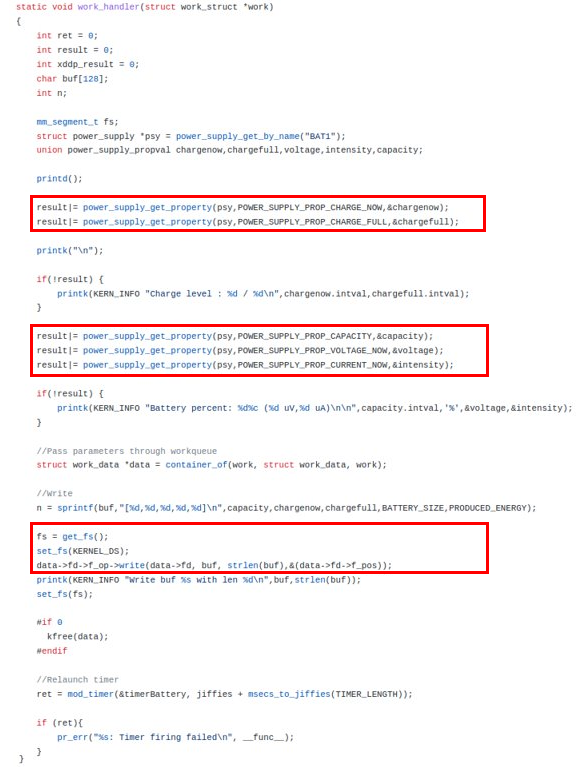
\includegraphics[scale=0.6]{work_task.png}
    	\caption{Work task handler for battery Linux module}
    	\end{figure} \newline
	  
  	\end{itemize}
	    
         
	    
	
	We also provide a fake battery module, initially retrieved from this repository : https://github.com/hoelzro/Linux-fake-battery-module \newline and whose purpose is to simulate the dynamic behaviour of a battery (Adaptation and more details \href{https://github.com/skyultime/M2_ERTS_Project_Xenomai_edh/tree/dev/SourceCode/fakeBatteryModule}{here})


%%%%%%%%%%%%%%%%%%%%%%%%%%%%%%%%%%%%%%%%%%%%%%%%%%%%%%%%%%%%%%%%%%
\newpage
\section{EDH over Xenomai}
\vspace{4cm}
    
    Now let's have a look to the implementation of ED-H over Xenomai. 3 steps are needed in order to modify the Xenomai source code (starting from a working Xenomai with EDF installation):
    \begin{enumerate}
        \item Add socket binding on XDDP port 0 to Xenomai source code to retrieve battery data
        \item Modify scheduler algorithm to select next task to run to match ED-H constraints (following the document available \href{https://hal.archives-ouvertes.fr/hal-02058575}{here}). 
        \item Modify alchemy API to match ED-H needs.
        
    \end{enumerate}
	\subsection{XDDP interdomain communication to gather battery data} \label{xddp}
	  \textbf{Please Keep in mind that this part is in devevlopment and  may evolve in the future.}
        
        As seen in the previous section, we have a linux module which can be load at boot. This module send battery informations to a RT tasks through the port 0.
        
        However in order for the module to access the port 0, we need to create a RT tasks in order to create a socket on minor 0.This RT tasks must be created without disturbing ED-H scheduling. To do this a first simple idea could be to add an additional task dedicated to open socket and receive battery information directly in user space. This idea isn't optimal. \newline Indeed to have a better integration of this RT tasks in xenomai source code, a second idea could be to add this RT task after Xenomai initialization ended.\newline
        
        To do this, we have created a couple file \textbf{batt.c/.h} directly in Cobalt directory and available \href{https://github.com/skyultime/Xenomai-EDH/blob/final_version/kernel/cobalt/batt.c}{here}
        Here is some useful information to understand the interest of theses files :
        \begin{itemize}
            \item To use \textbf{socket(), bind(), write(),read()...} functions, you need to add \textbf{rtdm} or \textbf{rtdm\_dev} prefix according to Xenomai Posix API.
            \item \textbf{batt\_init()} is the entry point. Calling this function will create a RT task dedicated to create a socket and then bind the socket to the port 0.
            \item \textbf{rtdm\_task\_init()} is used to ease the creation of a RT tasks
        \end{itemize}
        
        The 2 figures below provide source code for \textbf{batt\_init()} function and his handler function (called 
        \textbf{rt\_batt\_loop()})
        
	    \newpage \begin{figure}[ht]
        \centering
    	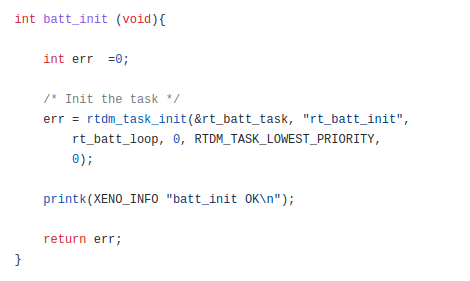
\includegraphics[scale=0.9]{battInit.png}
    	\caption{batt\_init function in batt.c}
    	\end{figure} \newline
    	
	    \begin{figure}[!h]
        \centering
    	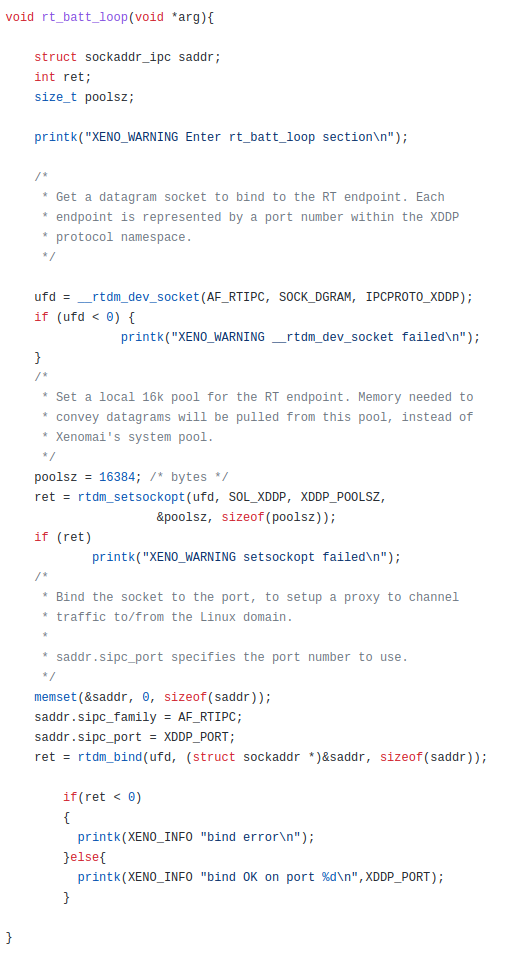
\includegraphics[scale=0.60]{battLoop.png}
    	\caption{RT tasks handler in batt.c }
    	\end{figure} \newline

        \newpage Problem to resolve : rtdm\_dev\_socket failed when calling the batt\_init() function from function \textbf{xenomai\_init} (see \href{https://github.com/skyultime/Xenomai-EDH/blob/final_version/kernel/cobalt/init.c}{here} for more details and figure below)
        
	    \begin{figure}[!h]
        \centering
    	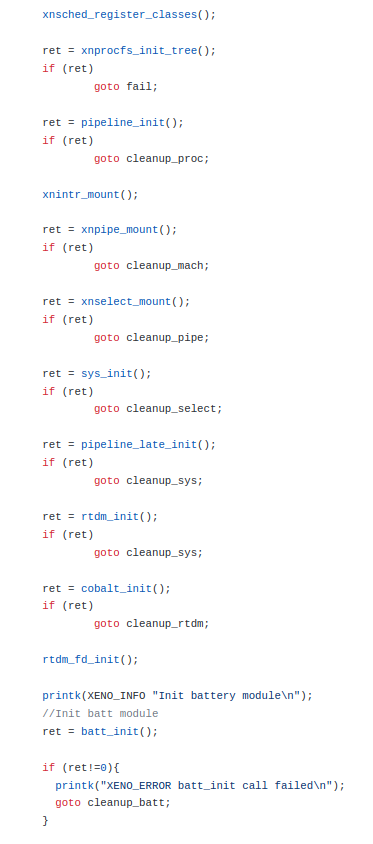
\includegraphics[scale=1]{initCall.png}
    	\caption{Call to batt\_init in xenomai\_init()}
    	\end{figure} \newline
    	 
	\newpage \subsection{Scheduler alg.} \label{slack_param}
	Let's now talk about how to modify the scheduler algorithm in order to follow ED-H constraints.
	
	When we use EDF policy or a round-robin policy, the function \textbf{xnsched\_pick\_next()} available \href{https://github.com/skyultime/Xenomai-EDH/blob/final_version/kernel/cobalt/sched.c}{here} is responsible to select the next task to be executed (depending on priority or deadlines). If we have at least one task ready to be executed, this task will  be executed and the CPU will always be loaded. In case we use the ED-H policy, sometimes we want the system to stay IDLE (we need to keep selecting the IDLE task for a given time) in order for the battery to be filled again.\newline
	
	To do this, we add few modifications to the function \textbf{xnsched\_pick\_next()} :
	
	\begin{itemize}
	    \item First we need to check the data \textbf{policy} of each task. Among all ready tasks, if we found a task with a \textbf{policy} equal to \textbf{EDH\_ALAP} or \textbf{EDH\_ASAP}, we need so to schedule the tasks set using ED-H policy. 
	    
	    \begin{figure}[ht]
        \centering
    	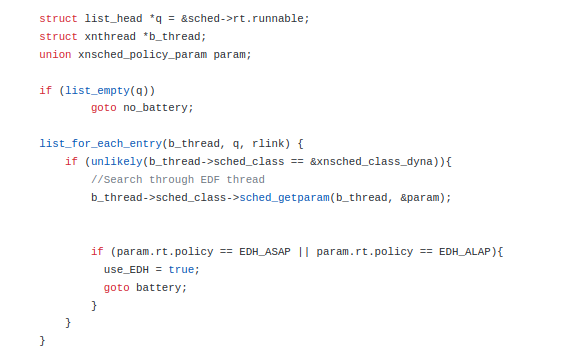
\includegraphics[scale=1]{EDH?.png}
    	\caption{1st modification in function \textbf{xnsched\_pick\_next()}}
    	\end{figure} \newline
	    
	    \newpage \item We retrieve battery data (from XDDP port 0) and we compute then slack\_energy and slack\_time for each ED-H tasks.
	    
	    As you can see on the figure below, slack\_energy and slack\_time are not yet computed.
	    
	    \begin{figure}[!h]
        \centering
    	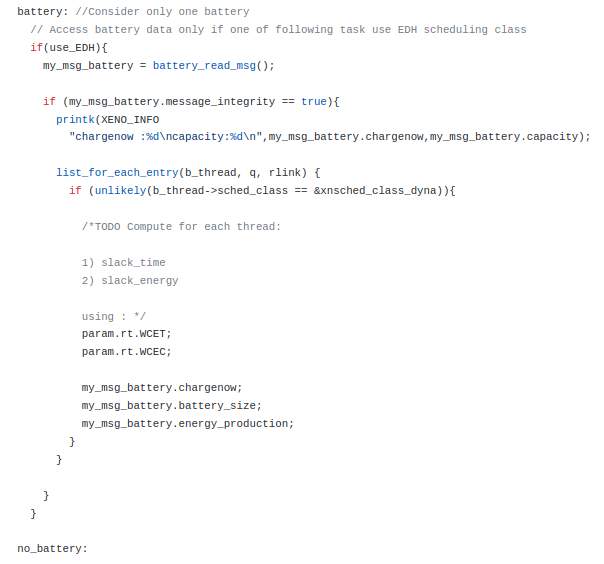
\includegraphics[scale=1]{batteryData.png}
    	\caption{2nd modification in function \textbf{xnsched\_pick\_next()}}
    	\end{figure} \newline
	    
	    \newpage \item We follow rules from the figure below. We have 2 possibility : execute a ready task from tasks set (could be the same running tasks) or execute the IDLE task.
    	
	    \begin{figure}[ht]
        \centering
        \begin{minipage}{0.45\textwidth}
            \centering
            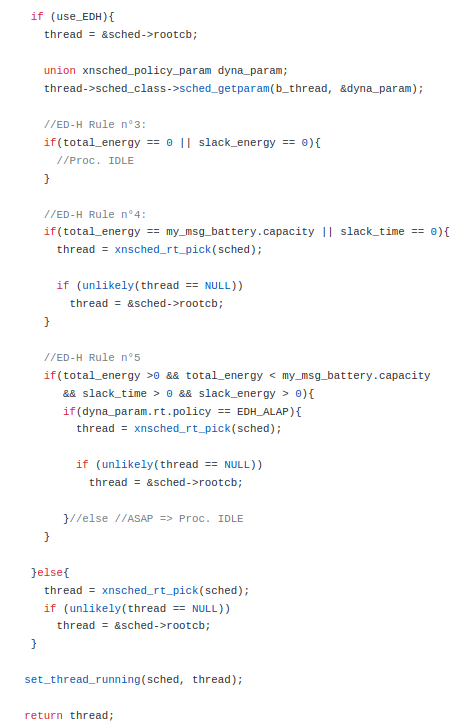
\includegraphics[width=1.2\textwidth]{EDH_rules.png} % first figure itself
            \caption{3rd modification in function \textbf{xnsched\_pick\_next()}}
        \end{minipage}\hfill
        \begin{minipage}{0.45\textwidth}
            \centering
            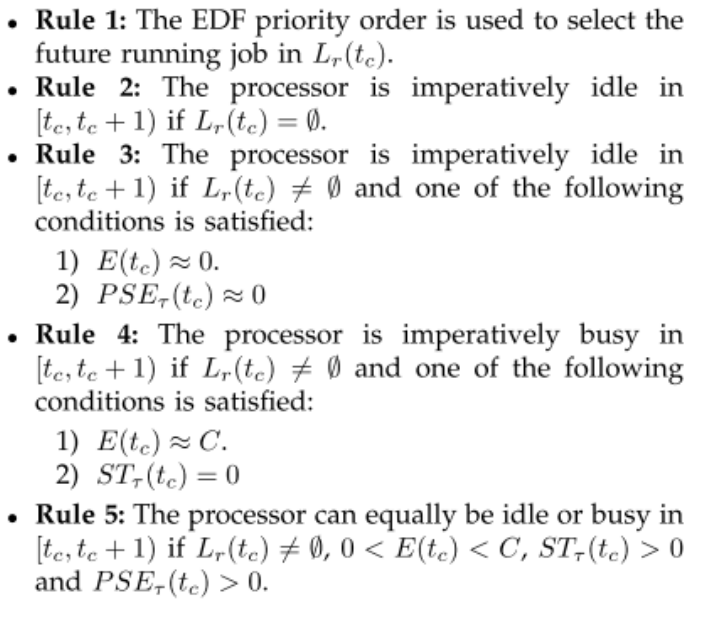
\includegraphics[width=1.2\textwidth]{EDH_rulesTheory.png} % second figure itself
            \caption{ED-H rules to respect}
        \end{minipage}
    \end{figure} \newline

	\end{itemize}
	
	\newpage \newpage \subsection{Alchemy API modifications}
	
	Initially, the alchemy API allow us to create RT task using round-robin scheduler. For this purpose, one of the parameters of the function \textbf{rt\_task\_create} is the priority. For EDF and ED-H we don't need it anymore. On top of this, we need more parameters.\newline
	
	We need so for each task:
	\begin{itemize}
	    \item EDF policy : the \textbf{deadline} of the task 
	    \item ED-H policy : \textbf{WCET},\textbf{WCEC} of the task (battery information are directly provided from the XDDP port).
	    
	    We add so another function, called \textbf{rt\_task\_dyna}, in order to create EDF/ED-H task. (same idea for \textbf{rt\_task\_spawn\_dyna}). This \href{https://github.com/skyultime/Xenomai-EDH/blob/final_version/include/alchemy/task.h}{function} owns all parameters mentioned above.
	    
	     \begin{figure}[!h]
        \centering
    	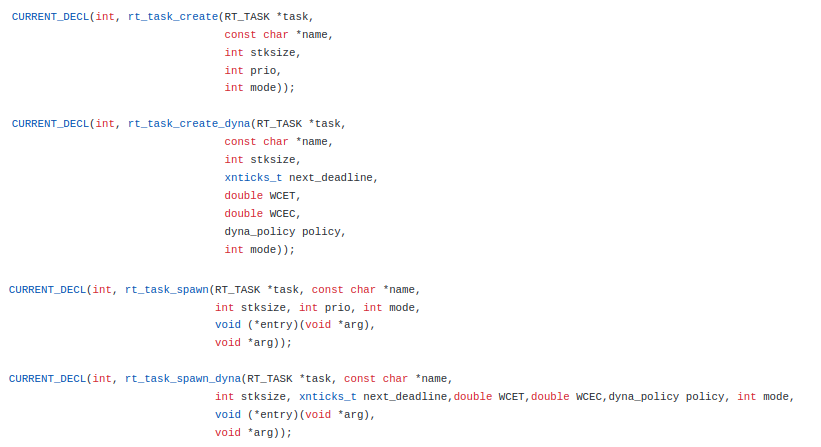
\includegraphics[scale=0.6]{alchemyAPI.png}
    	\caption{Alchemy API for task creation in file task.h}
    	\end{figure} \newline
	    
	    Lastly, in order to know if we want to schedule tasks using ED-H or EDF, we add an extra parameter, policy. The \href{https://github.com/skyultime/Xenomai-EDH/blob/final_version/include/cobalt/uapi/sched.h}{structure} is presented below :
	    
	     \begin{figure}[!h]
        \centering
    	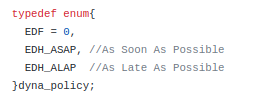
\includegraphics[scale=1]{dyna_policy.png}
    	\caption{Structure dyna\_policy in file uapi/sched.h}
    	\end{figure} \newline
	    
	\end{itemize}
	
	Without entering into details of implementation, don't hesitate to look at this commit for example : \href{https://github.com/skyultime/Xenomai-EDH/commit/f339c141faf314a96725899d3941c65e162457d1}{commit link}
	Looking at this commit, you can see which files are needed to be modified in order to adapt Xenomai source code and more particularly the alchemy API.  
	
	\newpage \subsection{Remaining tasks and ameliorations} \label{remaining}
	Here we will first list all the remaining tasks to achieve in order to have a working EDH policy over Xenomai
	\begin{itemize}
	    
	    \item Compute slack\_time and slack\_energy for each task in section \ref{slack_param}. To do this, you can have a look in section \ref{SlackMethodEnergy} and section \ref{SlackMethodTime} to know how to compute these values.
 	    
 	    \item Solve problem to create a socket on port 0 to gather battery information from RT context (in primary domain). (cf  section \ref{xddp})
 	    
	    \item Test ED-H source code implementation over Xenomai
	    
	\end{itemize}
	
	To test ED-H source code, you can use the cheddar simulator to compare your results. You can also use the fake linux battery module to simulate dynamic behaviour of any kind of battery. Finally, you can have a look \href{https://github.com/skyultime/M2_ERTS_Project_xenomai_edh/tree/dev/Tests/EDHonXenomai/edhAsserts}{here} in order to ease the creation of tasks to be scheduled using ED-H policy (Still need few minor adaptations to be used).
	
	\newpage
%%%%%%%%%%%%%%%%%%%%%%%%%%%%%%%%%%%%%%%%%%%%%%%%%%%%%%%%%%%%%%%%%%
\newpage
\section{Planning \& project evolution}
\vspace{4cm}
	\subsection{Planning}
	
	In this section we will compare the provisional planning (initialy created on October, the 13th) with the effective planning.
	
     \begin{figure}[!h]
        \hspace{-2cm}
        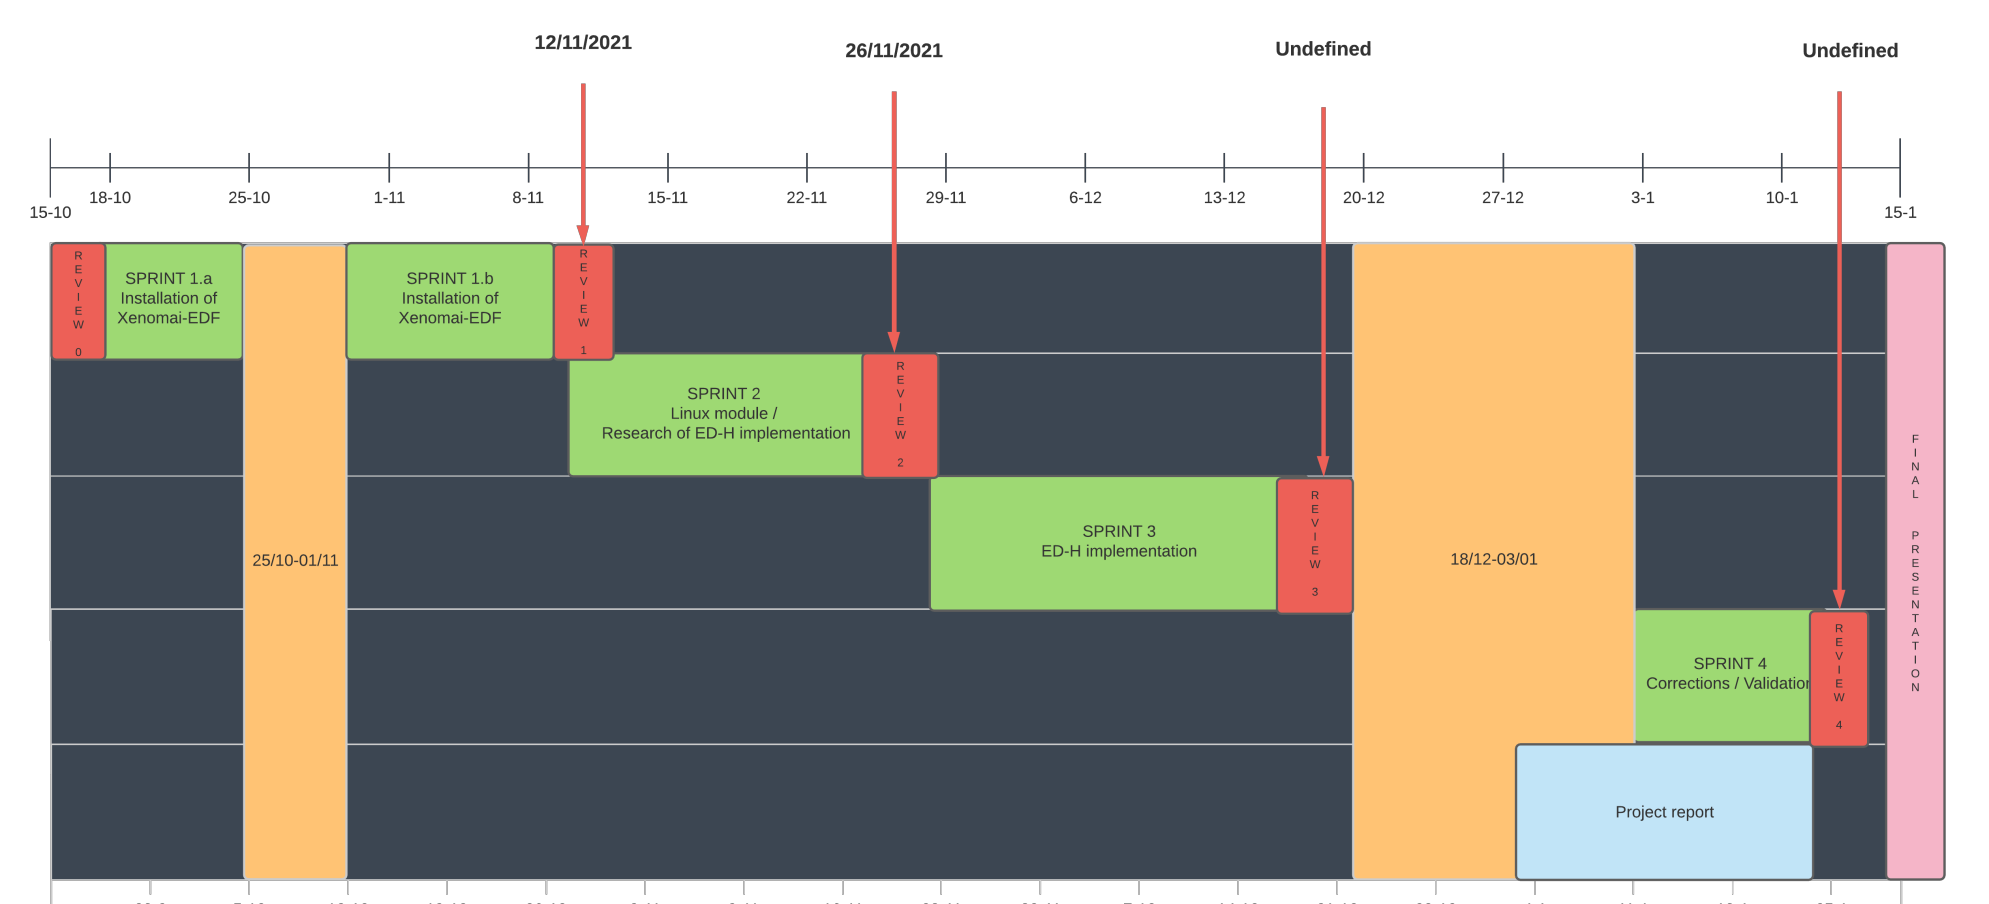
\includegraphics[width=20cm,height=6cm]{provisionalPlanning.png}
        \caption{Provisional planning}
    \end{figure} \newline
    
     \begin{figure}[!h]
        \hspace{-2.5cm}
        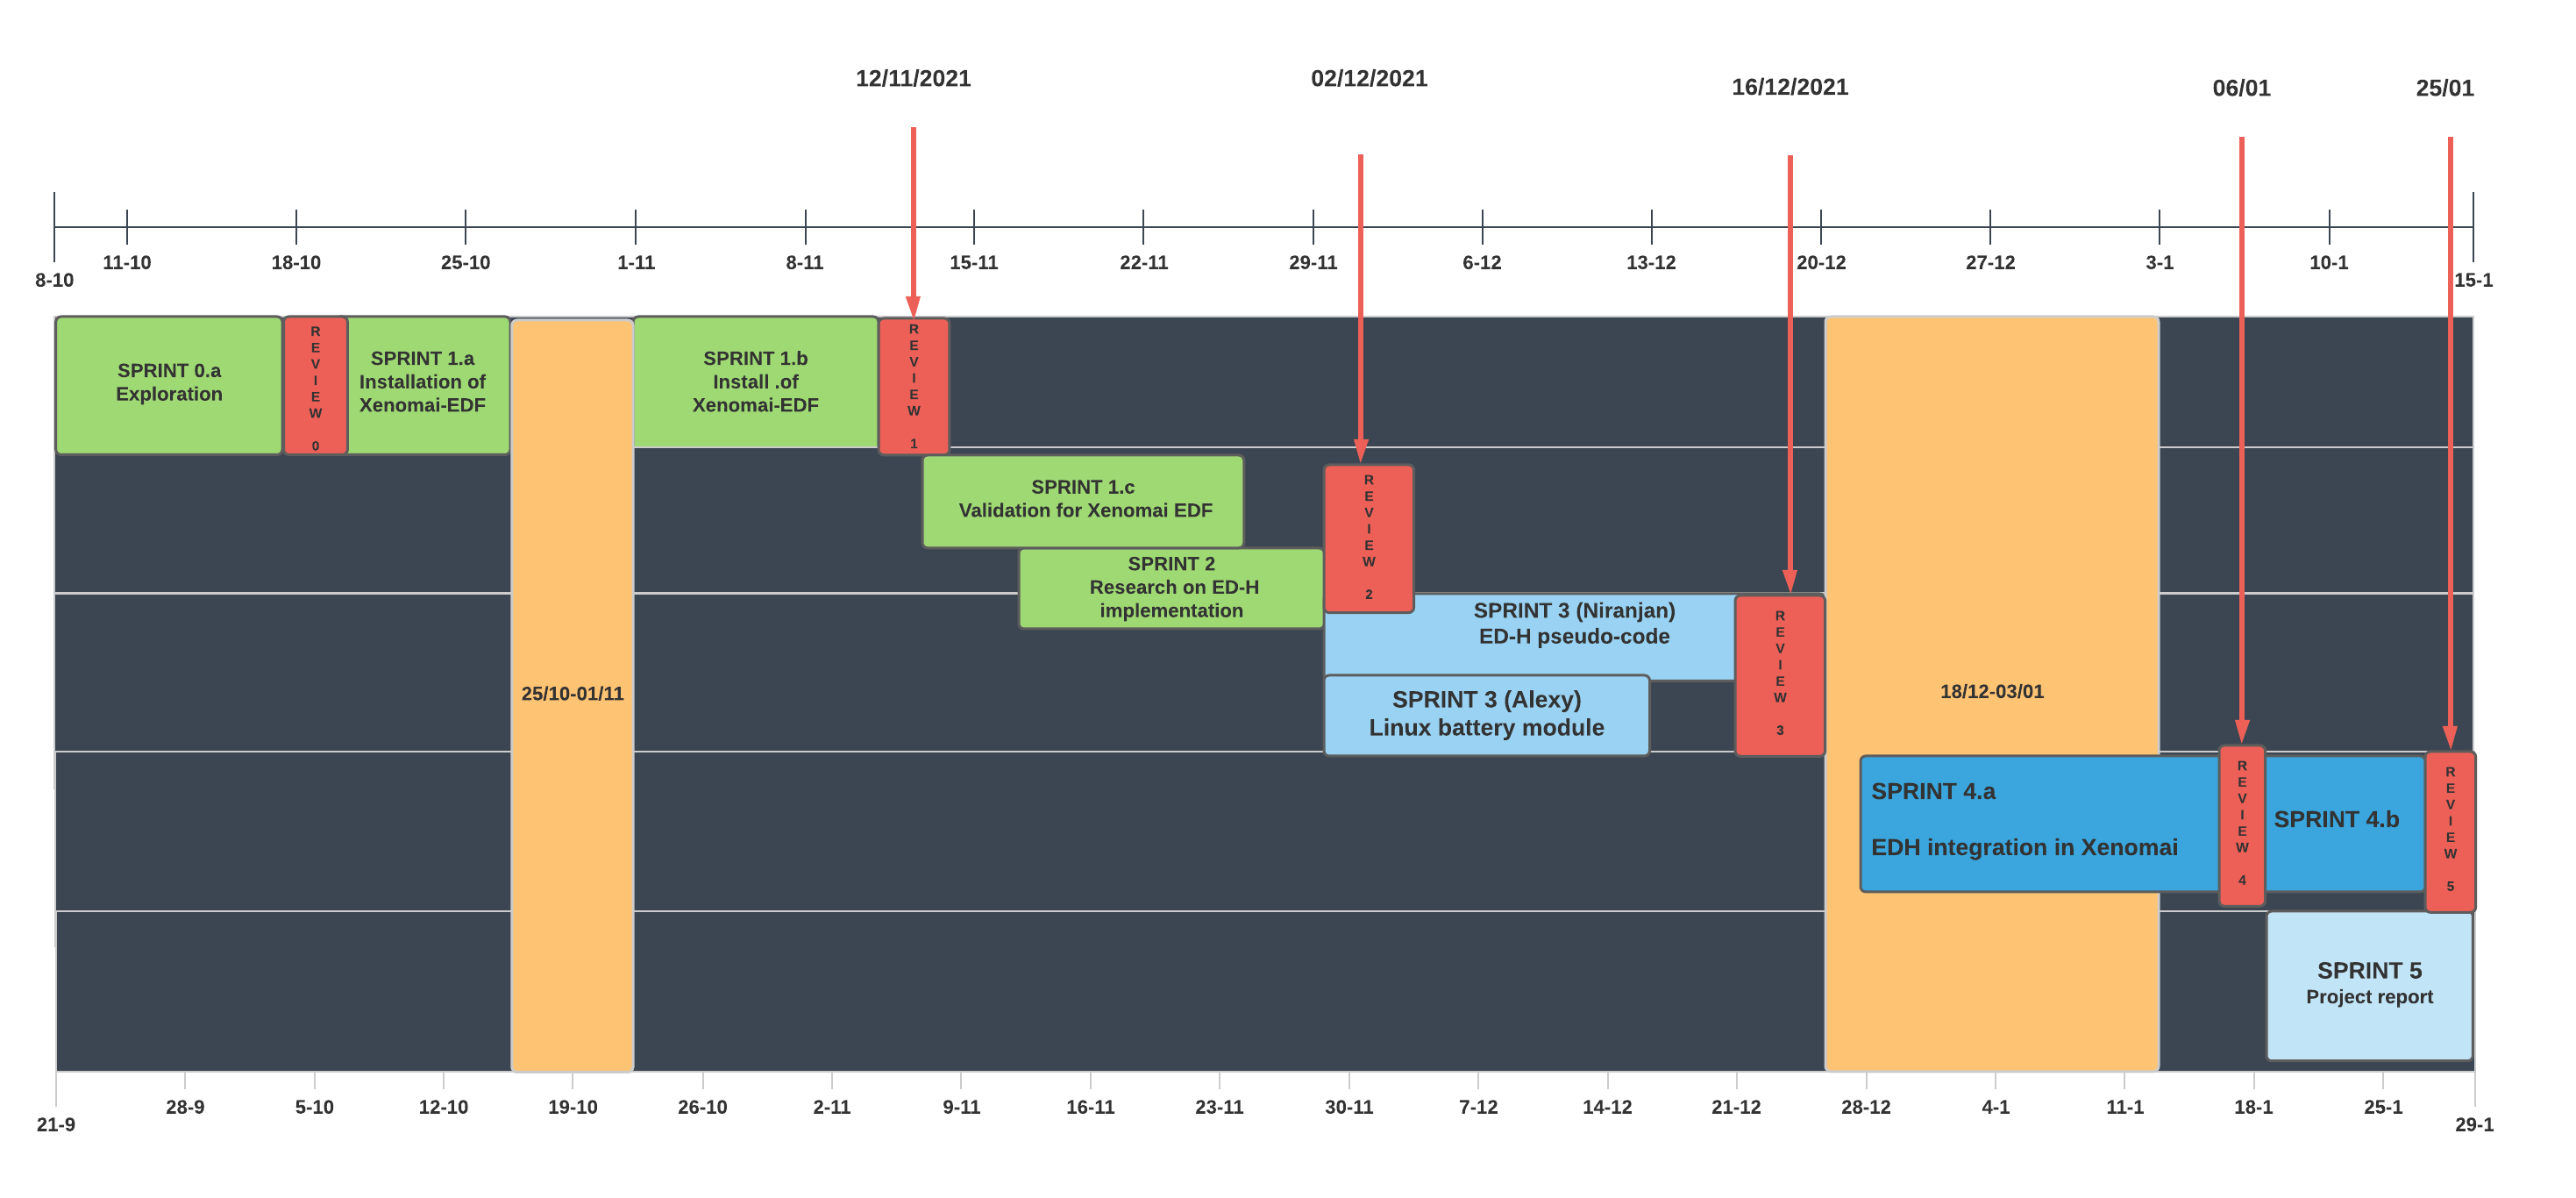
\includegraphics[width=20cm,height=8cm]{PFE - Plannings.png}
        \caption{Effective planning}
    \end{figure} \newline
	
	\newpage
	
	As we can see, we didn't take into account the validation of EDF source code over Xenomai in the provisional planning. Indeed the source code files for EDF implementation over Xenomai have had to be reviewed to solve compilation errors/warnings during the linux kernel compilation. On top of that, we have had to assert EDF is working correctly over Xenomai (cf section \ref{validation}). All these have contribute to postponed by 2 weeks the ED-H implementation (really begin at \textbf{Sprint 3} in figure 24 instead of \textbf{Sprint 2} in figure 23)
	
	\subsection{Progress}
	
	A short overview of our progress in this project is presented below (figure extract from the final review, available \href{https://github.com/skyultime/M2_ERTS_Project_xenomai_edh/tree/dev/Doc/PwpSlides/finalReview}{here})\newline
	
     \begin{figure}[!h]
        \hspace{-1cm}
        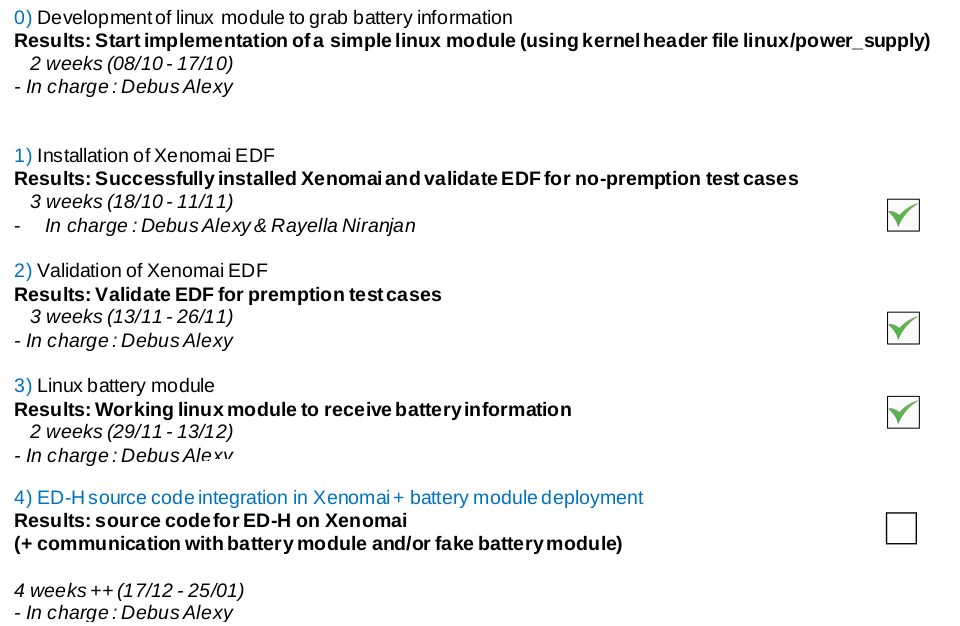
\includegraphics[scale=0.7]{overProgress.png}
        \caption{Overall progress in project}
    \end{figure} \newline \newline

	On top of that, please refer to the previous section \ref{remaining} to have a global overview of remaining jobs.
	Keep in mind the 2 remaining tasks in order to finish EDH implementation over EDH:
	
	\begin{itemize}
	    \item Compute slack\_energy and slack\_time for each task (section \ref{slack_param})
	    \item Ensure XDDP communication working (battery informations retrieve from a RT task, section \ref{xddp})
	    
	\end{itemize}
	
%%%%%%%%%%%%%%%%%%%%%%%%%%%%%%%%%%%%%%%%%%%%%%%%%%%%%%%%%%%%%%%%%%
\newpage

\section{References}
\vspace{4cm}
\bibliographystyle{ieeetr}
\bibliography{references}

\newpage

\thispagestyle{empty}
\listoffigures
\listoftables

%%%%%%%%%%%%%%%%%%%%%%%%%%%%%%%%%%%%%%%%%%%%%%%%%%%%%%%%%%%%%%%%%%
\end{document}





















